\documentclass[doctor,korean,final]{kmu}
\special{papersize=182mm,257mm}

\usepackage{times}
\usepackage{CJKutf8}
\usepackage{mathrsfs}
\usepackage{textcomp}
\usepackage{verbatim}
\usepackage{amsmath}
\usepackage{amsfonts}
\usepackage{xspace}
\usepackage{xcolor}
\usepackage{url}
\usepackage{balance}
\usepackage{booktabs}
\usepackage{multirow}
\usepackage{rotating}
\usepackage{fancyvrb}
\usepackage{lastpage}
\usepackage{alltt}
\usepackage{etoolbox}
\usepackage{cleveref} % After hyperref, listings
\usepackage{fancyhdr}
\usepackage{listings}

\usepackage{macro}
\newenvironment{CompactItemize}{\begin{itemize}}{\end{itemize}}
\def\code#1{{\texttt{#1}}}


\usepackage{caption}
\usepackage{subcaption}

\usepackage{tikz}
\usetikzlibrary{shapes,snakes}


\usepackage{amsmath}
\usepackage{amssymb}
\usepackage{wasysym}

%The given symbol or text (\text{mytext}) in a circle
%To be used always in math mode
\newcommand{\circlesign}[1]{ 
    \mathbin{
        \mathchoice
        {\buildcirclesign{\displaystyle}{#1}}
        {\buildcirclesign{\textstyle}{#1}}
        {\buildcirclesign{\scriptstyle}{#1}}
        {\buildcirclesign{\scriptscriptstyle}{#1}}
    } 
}


\newcommand\buildcirclesign[2]{%
    \begin{tikzpicture}[baseline=(X.base), inner sep=0, outer sep=0]
    \node[draw,circle] (X)  {\ensuremath{#1 #2}};
    \end{tikzpicture}%
}

\definecolor{lbcolor}{rgb}{0.9,0.9,0.9}
\lstset{
    tabsize=2,    
    language=C,
    basicstyle=\footnotesize\ttfamily,
    upquote=true,
    aboveskip={1.5\baselineskip},
    columns=fixed,
    extendedchars=false,
    showtabs=false,
    showspaces=false,
    showstringspaces=false,
    identifierstyle=\ttfamily,
    keywordstyle=\color[rgb]{0,0,1},
    commentstyle=\color[rgb]{0.026,0.112,0.095},
    stringstyle=\color[rgb]{0.627,0.126,0.941},
    numberstyle=\color[rgb]{0.205, 0.142, 0.73},
}


\usepackage{colorhist}
 
\usepackage{minted}
\usepackage{pdfpages}



% 본문 시작
\begin{document}

% 표목차 (List of Tables) 생성
%\listoftables

% 그림목차 (List of Figures) 생성
%\listoffigures

% 위의 세 종류의 목차는 한꺼번에 다음 명령으로 생성할 수도 있습니다.
%\makecontents
%% 한글로 쓴 논문에는 본문에 영문 글자를 쓰지 않는다. 다만, 꼭 필요할 때에는 ‘한글 낱말 (영문 낱말)’ 꼴로 적는다.
%% 이하의 본문은 LaTeX 표준 클래스 report 양식에 준하여 작성하시면 됩니다.
%% 하지만 part는 사용하지 못하도록 제거하였으므로, chapter가 문서 내의
%% 최상위 분류 단위가 됩니다.
%% You cannot use 'part'

%본문을 한글로 작성할 때 머릿말로 시작을 하시는 게 좋습니다. \cite{FD1}
%인용은 다음과 같이 합니다 \cite{RVP1}-\cite{ML2}.
%인용은 뒤에 인용을 쓰는 칸이 있습니다. 참고하여서 인용하시길 바랍니다 \cite{SOCA2,EF2}.
%한글 논문에는 영어를 쓰지 마시기 바랍니다. 

\newif\ifkor
\kortrue 

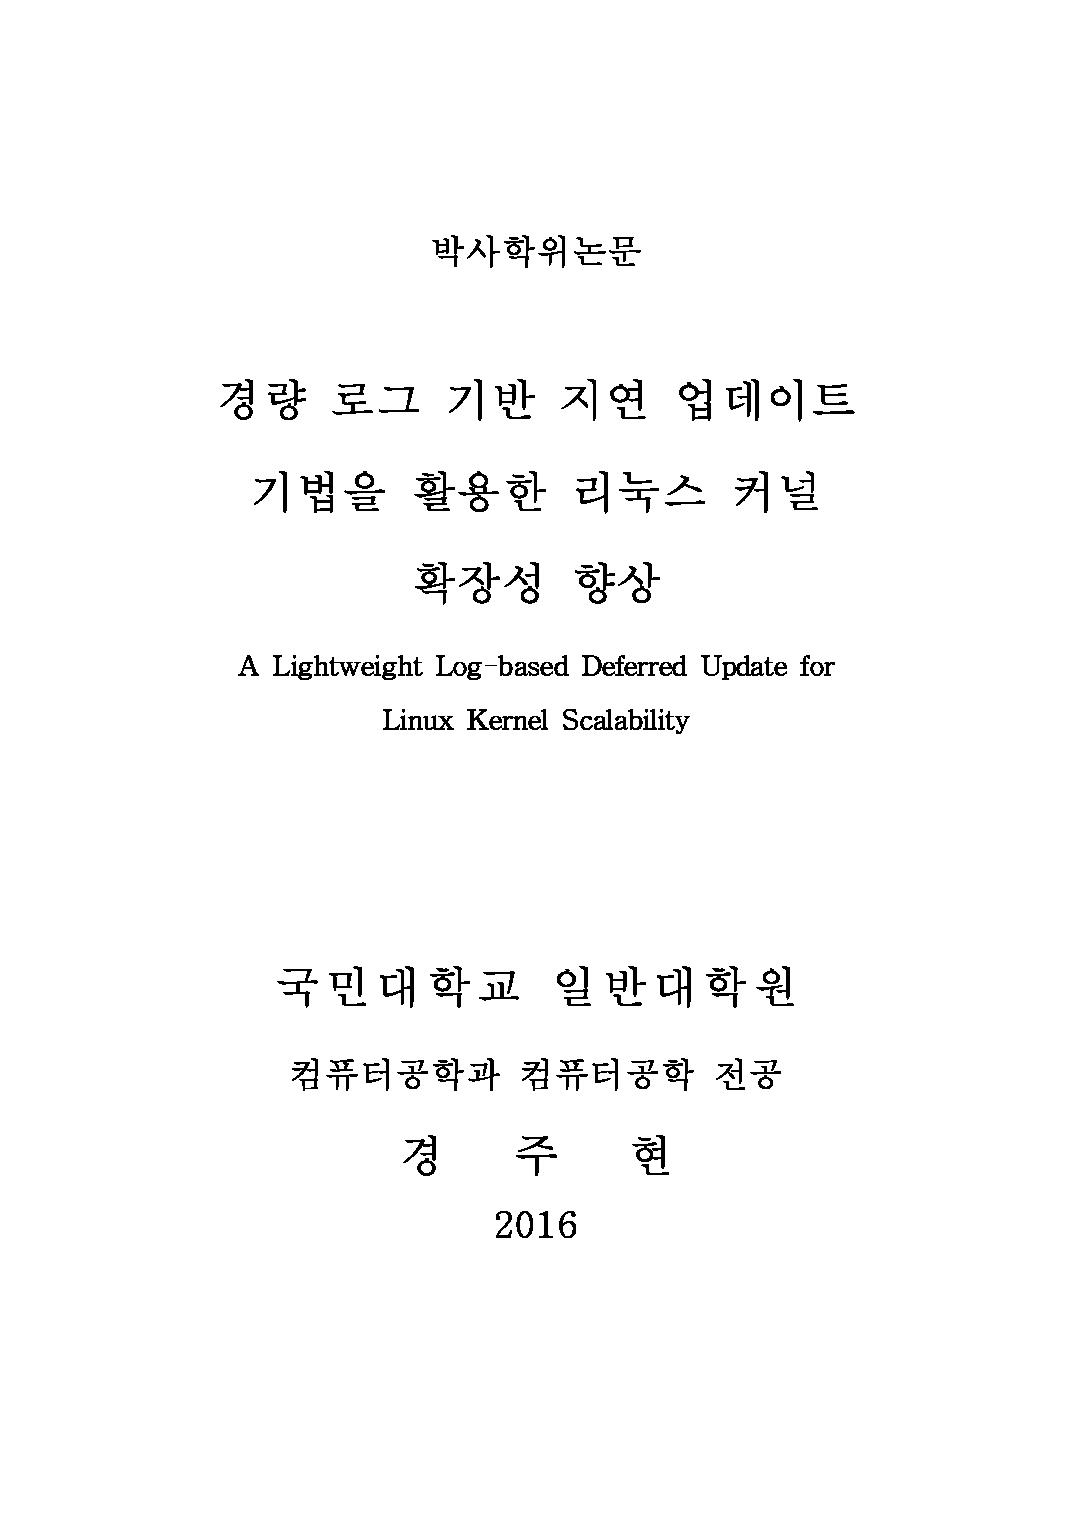
\includepdf[pages=1]{title_1.pdf}
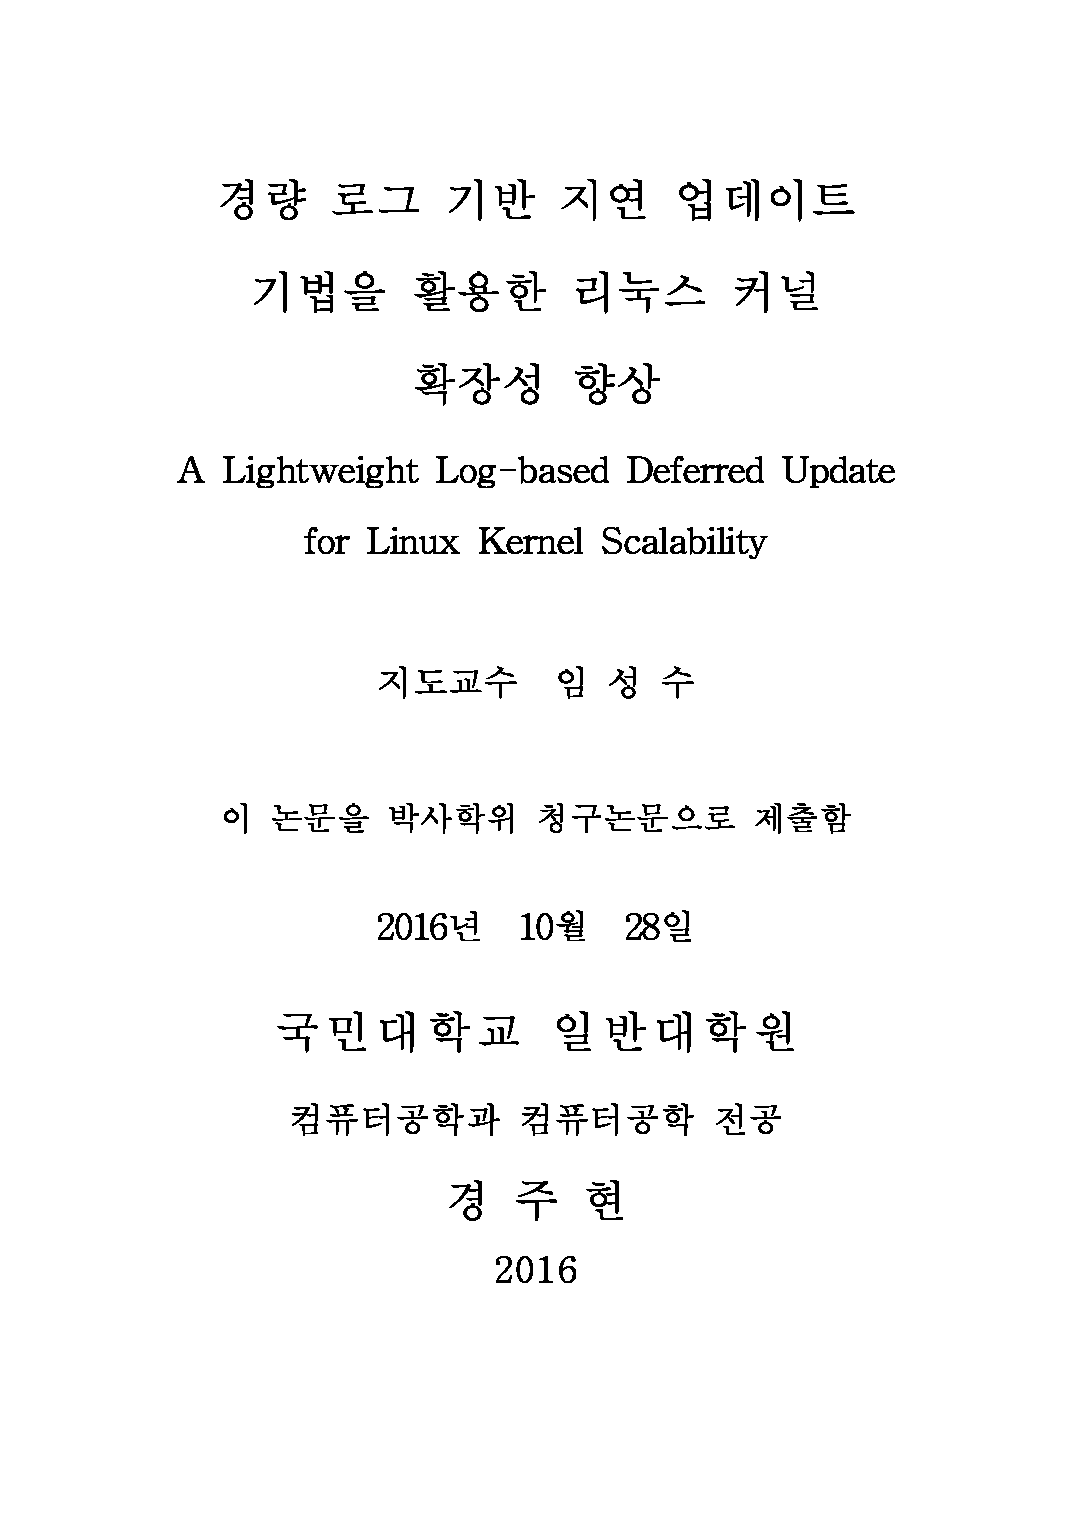
\includepdf[pages=1-2]{title_2.pdf}


\pagenumbering{roman}                         % roman 페이지번호로 복원
\setcounter{page}{\value{pagemarker}}         % pagemarker에 저장된 값으로

% 목차 (Table of Contents) 생성
\tableofcontents
% 그림목차 (List of Figures) 생성
\listoffigures
% 표목차 (List of Tables) 생성
%\listoftables

\pagenumbering{roman}                         % roman 페이지번호로 복원
\setcounter{page}{\value{pagemarker}}         % pagemarker에 저장된 값으로
\addcontentsline{toc}{content}{요약}% 목차(TOC)에 추가
\label{paperlastromanpagelabel}     % <-- 추가 부분: 마지막 페이지 위치 지정

\hfill \break


\noindent
\Large{\textbf{국문 요약}}
\newline
\\
\noindent
\Large{\textbf{경량 로그 기반 지연 업데이트 기법을 활용한 리눅스 커널 확장성 향상}}

\normalsize{
\hfill \break
\begin{center}
\raggedleft{국민대학교 일반대학원 컴퓨터공학과}\\
\end{center}

\begin{center}
\raggedleft{경주현}\\
\end{center}
\hfill \break

  공유 메모리 시스템 구조를 가지는 매니코어 시스템에서 성능 확장성은 매우 중요한 요소 중 하나이다.   
이러한 성능 확장성 중 운영체제의 성능 확장성은 시스템 전체에 영향을 준다. 
만약 운영체제가 확장성이 없다면 그 운영체제의 서비스를 이용하는 모든 응용프로그램은 확장성이 없게 된다.
이처럼 중요한 운영체제의 확장성 문제 중 업데이트 비율이 높은 자료구조를 위한 
로그 기반 동시적 업데이트 기법들이 그동안 연구되었다. 
이러한 로그 기반 동시적 업데이트 기법 중 하나는 
시스템에 전역 타임스탬프 카운터가 있다는 것을 가정하여 타임스탬프와 로그를 함께 저장하여 
사용한 방법이 있다. 
이 방법은 업데이트 연산이 많을 경우 굉장히 높은 확장성을 가진다. 
하지만 NUMA 구조를 가지는 매니코어 시스템에서 보장된 동기화된 
전역 타임스탬프 카운터는 아직 없는 현실적인 문제점을 가지고 있다.

본 논문은 하드웨어 적으로 지원하지 않는 동기화된 전역 타임스탬프 카운터 기법의 현실적인 문제점을 
해결하기 위해, 새로운 동시적 업데이트를 위한 경량 로그 기반 지연 업데이트 방법인 
LDU(Lightweight log-based Deferred Update)를 개발하였다.
LDU는 타임스탬프 카운터가 필요한 연산을 하드웨어 동기화 기법을 사용하여 
로그가 발생하는 순간 제거하고 불필요한 로그를 제거하는 방법이다. 
이를 통해 동기화된 타임스탬프 카운터를 완벽 제거하였으며, 동시에 동시적 업데이트 방법들의 문제점인
캐시 일관성 트래픽 문제를 해결하였다.

본 연구에서는 이러한 LDU를 리눅스 커널 내부 자료구조 중 높은 업데이트 비율 때문에 성능 확장성 
문제를 야기하는 가상 메모리 시스템에 적용하였고, 이를 통해 확장성을 향상 시켰다.
리눅스 커널 4.5-rc4에 구현하였으며, 120코어 매니코어 시스템에서 확장성 벤치마크를 대상으로 
1.5배에서 2.7배까지 성능 향상을 이루었다. 

%To overcome the scalability degradation problem, we introduce a lightweight
%log-based deferred update method, combining the log-based concepts in the
%distributed systems and the minimal hardware-based synchronization in the
%shared memory systems.
%The main contributions of the proposed method are:(1) we propose a lightweight
%log-based deferred update method, which can eliminate synchronized time-stamp
%counters that limits the performance scalability;and (2) we implemented the
% proposed method in the Linux 4.5-rc6 kernel for two representative data
% structures (anonymous reverse mapping and file mapping) and evaluated the
%performance improvement due to our proposed novel light weight update method.
%Our evaluation study showed that application of our method could
%achieve from 1.5x through 2.7x performance improvements in 120 core
%systems.
}


\newpage \setcounter{pagemarker}{\value{page}}% pagemarker에 다시 저장
\pagenumbering{arabic}                        % arabic 페이지번호로 재시작

\chapter{서론}
\section{개요} \label{sec:intro}

%$$$$$$$$$$$$$$$$$$$$$$$$$$$$$$$$$$$$$$$$$$$$$$$$$$$$$$$$$$$$$$$$$$$$$$$$$$$$$$$$
%$$$$$$$$$$$$$$$$$$$$$$$$$$$$$$$$$$$$$$$$$$$$$$$$$$$$$$$$$$$$$$$$$$$$$$$$$$$$$$$$
%Background
%$$$$$$$$$$$$$$$$$$$$$$$$$$$$$$$$$$$$$$$$$$$$$$$$$$$$$$$$$$$$$$$$$$$$$$$$$$$$$$$$
%Achieving performance scalability has been a most important factor in 
%highly parallel systems with many cores (e.g., over 100 cores).
성능에 대한 확장성(Scalability)은 100코어 또는 1000코어 이상으로 구성된 
매니코어(Many-core) 시스템에서 가장 중요한 요소이다. 
%The performance scalability of a whole system is naturally limited by 
%scalability of underlying operating system kernel; Linux kernel has been 
%widely considered in ordinary systems.
전체 시스템의 성능 확장성은 일반적으로 운영체제의 커널(Kernel) 때문에 제한을 받는다.
이러한 운영체제 커널 중 가장 많이 사용되는 것은 리눅스(Linux) 커널이다. 
그 이유는 리눅스 커널은 멀티코어에 최적화가 되어 있기 때문이다.
%Previous research revealed that Linux kernel has significant problems limiting
%performance scalability in many core
% systems~\cite{SilasBoydWickizer2010LinuxScales48}~\cite{Changwoo2016UMSF} and
% the major sources of the problems are update lock contention in a few kernel data structures~\cite{mckenney2011parallel}~\cite{Matveev2015RLU}.
하지만 이렇게 멀티코어에 최적화된 리눅스 커널도 매니코어 시스템에서는 여전히 
성능에 대한 확장성에 문제가
있다~\cite{SilasBoydWickizer2010LinuxScales48}~\cite{Changwoo2016UMSF}.
확장성 문제 중 가장 큰 문제는 커널의 자료구조 중 업데이트 락(Lock) 경쟁에 대한
문제 때문이다~\cite{mckenney2011parallel}~\cite{Matveev2015RLU}.



%$$$$$$$$$$$$$$$$$$$$$$$$$$$$$$$$$$$$$$$$$$$$$$$$$$$$$$$$$$$$$$$$$$$$$$$$$$$$$$$$
%$$$$$$$$$$$$$$$$$$$$$$$$$$$$$$$$$$$$$$$$$$$$$$$$$$$$$$$$$$$$$$$$$$$$$$$$$$$$$$$$
%Problem general
%$$$$$$$$$$$$$$$$$$$$$$$$$$$$$$$$$$$$$$$$$$$$$$$$$$$$$$$$$$$$$$$$$$$$$$$$$$$$$$$$
%Early research accomplishments regarding the update serialization problems
%include a number of concurrent
%update
% methods~\cite{Arbel2014ConcurrentRCU}~\cite{Matveev2015RLU}~\cite{Dodds2015SCT}.
이처럼 업데이트 직렬화(Serialization) 문제를 해결하기 위해 여러 동시적 업데이트(Concurrent Update)
 방법들이 연구되고
 있다~\cite{Arbel2014ConcurrentRCU}~\cite{Matveev2015RLU}~\cite{Dodds2015SCT}.
%Such research provides bases to solve the update serialization problems, but
%does not effectively handle serious scalability bottleneck for update-heavy
% data structures.
동시적 업데이트 방법을 사용하여 업데이트 직렬화 문제를 해결하는 연구들은 
업데이트 비율에 따라 많은 성능 차이를 보인다.
이러한 방법들은 높은 업데이트 비율을 가진 자료 구조 때문에 발생하는 확장성 문제에 
대해서는 여전히 효율적이지 않다.  
%Log-based algorithms~\cite{Hendler2010FC}~\cite{SilasBoydWickizerPth}
%have been proposed to solve this update serialization problem by reducing cache
% coherence-related overheads for update-heavy data structures.
높은 업데이트 비율을 가진 자료에 대한 해결책 중 하나는 캐시 통신 병목(cache communication bottleneck)
현상을 줄인 로그 기반(log-based) 알고리즘~\cite{Hendler2010FC}~\cite{SilasBoydWickizerPth}을
사용하는 것이다.
%When update operations occur, log-based algorithm logs the update
%operation and applies all operation logs to the data structure
%before read operation, so readers can read up to date data structure in a way
%similar to CoW(Copy On Write)~\cite{PaulDetailLWN}~\cite{Morrison2016SSM}.
로그 기반 알고리즘은 업데이트가 발생하면, 자료구조의 업데이트 명령(update operation)을
퍼코어(per-core) 또는 원자적(atomic)으로 로그로 저장하고 읽기 명령(read operation)을 수행하기
 전에 저장된 로그를 수행하는 것이다.
따라서, 리더(reader)는 최신 데이터를 읽게 되며, 이것은 마치 CoW(Copy on Write)와
유사하다~\cite{PaulDetailLWN}~\cite{Morrison2016SSM}.

%$$$$$$$$$$$$$$$$$$$$$$$$$$$$$$$$$$$$$$$$$$$$$$$$$$$$$$$$$$$$$$$$$$$$$$$$$$$$$$$$
%$$$$$$$$$$$$$$$$$$$$$$$$$$$$$$$$$$$$$$$$$$$$$$$$$$$$$$$$$$$$$$$$$$$$$$$$$$$$$$$$
%Problem 
%$$$$$$$$$$$$$$$$$$$$$$$$$$$$$$$$$$$$$$$$$$$$$$$$$$$$$$$$$$$$$$$$$$$$$$$$$$$$$$$$
%Among the log-based methods,
%S. Boyd-Wickizer \textit{et al.} proposed OpLog~\cite{SilasBoydWickizerPth},
% where each update operation generates a log with synchronized time-stamp counters
%and serialization of the logs based on the time-stamps solves the scalability
%bottleneck for update-heavy data structures: 
%the loggings are performed on to per-core memory instead of shared memory and
%thus eliminates cache communication overhead.
S. Boyd-Wickizer et al.는 동기화된 타임스탬프 카운터(synchronized timestamp counters) 기반의
퍼코어 로그를 활용하여 높은 업데이트 비율을 가진 자료구조를 대상으로 동시적 업데이트 문제를
해결함과 동시에 캐시 병목현상(cache communication bottleneck)을
줄였다~\cite{SilasBoydWickizerPth}.
동기화된 타임스탬프 카운터 기반의 퍼코어 로그를 활용한 동시적 업데이트방법은
업데이트 부분만 고려했을 때, 퍼코어에 데이터를 저장함으로 굉장히 높은 성능 확장성을
 가진다[].
%However, the OpLog still has problems in scalability since the synchronized
% time-stamp counters necessitates time-stamp merging and ordering processes leading to 
%performance scalability problems in high CPU core counts.
하지만 퍼코어 기반의 동기화된 타임스탬프 카운터를 사용한 방법은 결국 타임스탬프 병합(timestamp merging)
과 정렬(ordering) 작업을 야기한다.
만약 코어 수가 늘어 날 경우, 로그를 자료 구조에 적용하는 과정에서 타임스탬프(timestamp)
 때문에 발생하는 추가적인 순차적 프로세싱(sequential processing)이 요구된다.
이것은 결국 확장성과 성능을 저해한다. 


%$$$$$$$$$$$$$$$$$$$$$$$$$$$$$$$$$$$$$$$$$$$$$$$$$$$$$$$$$$$$$$$$$$$$$$$$$$$$$$$$
%$$$$$$$$$$$$$$$$$$$$$$$$$$$$$$$$$$$$$$$$$$$$$$$$$$$$$$$$$$$$$$$$$$$$$$$$$$$$$$$$
%Method
%$$$$$$$$$$$$$$$$$$$$$$$$$$$$$$$$$$$$$$$$$$$$$$$$$$$$$$$$$$$$$$$$$$$$$$$$$$$$$$$$
%
%We propose a novel lightweight log-based differed update method(\LDU) to
% achieve the maximum performance scalability for update-heavy data structures solving the 
%problems of sequential processing raised from the previous research:
%cache communication overhead in logging and time-stamp management cost during
% log ordering. 
%Such improved scalability could be achieved through combination of widely known 
%log-based concurrent update concept and our own way of efficient implementation
%methods of the log management scheme: log record slot reuse in the log queue
% and using minimal hardware-based synchronization
%method(compare and swap, test and set, atomic swap).
본 논문은 동기화된 타임스탬프 카운터를 이용함에 따라 생기는 추가적인 순차적 프로세싱(sequential processing) 문제를
해결하기 위해 공유 메모리 시스템을(shared memory system) 위한 새로운 LDU(Lightweight log-based
Deferred Update)를 개발하였다.
LDU는 타임스탬프 카운터가 필요한 명령어 로그(operation log)를 업데이트 순간 지우고,
 매번 로그를 생성하지 않고 재활용하는 방법이다.
이로 인해 동기화된 타임스탬프 카운터 문제와 캐시 커뮤니케이션 병목현상에 대한 문제를 동시에 해결하였다.
해결 방법은 분산 시스템(distributed system)에서 사용하는 동기화된 타임스템프 로그 기반의 
동시적 업데이트 방식과 최소한의 공유 메모리 시스템의 하드웨어 기반 동기화(hardware-based
synchronization) 기법(compare and swap, test and set, atomic swap)을 조합하여 동시적 업데이트
문제를 해결하였다.

이처럼 동기화된 타임스탬프 카운터를 제거함과 동시에, 캐시 커뮤니케이션 병목 현상을 줄인
LDU는 기존 로그 기반 알고리즘들의 장점들을 모두 포함할 뿐만 아니라 추가적인 장점을 가진다.
첫째로, 업데이트가 수행하는 시점 즉 로그를 저장하는 순간에는
 파인 그레인드 동기화 기술(fine-grained synchronization)이 필요가 없다.
따라서 동기화(synchronization) 오버헤드 없이 동시적 업데이트를 수행할 수 있다
둘째로, 저장된 업데이트 명령어 로그를 코스 그레인드 동기화 기술(coarse-grained synchronization)과 함께 하나의
코어에서 수행하기 때문에, 캐시 효율성이 높아진다~\cite{Hendler2010FC}.
다음으로, 기존 여러 자료구조에 쉽게 적용할 수 있는 장점이 있다.
게다가 마지막으로, 로그를 저장하기 전에 로그를 삭제하므로 더욱 빠르게 로그의 수를 줄일 수 있다. 

%$$$$$$$$$$$$$$$$$$$$$$$$$$$$$$$$$$$$$$$$$$$$$$$$$$$$$$$$$$$$$$$$$$$$$$$$$$$$$$$$
%$$$$$$$$$$$$$$$$$$$$$$$$$$$$$$$$$$$$$$$$$$$$$$$$$$$$$$$$$$$$$$$$$$$$$$$$$$$$$$$$
%Result
%$$$$$$$$$$$$$$$$$$$$$$$$$$$$$$$$$$$$$$$$$$$$$$$$$$$$$$$$$$$$$$$$$$$$$$$$$$$$$$$$

%To evaluate our approach, we applied the \LDU to Linux kernel reverse
%page mappings(anonymous page mapping, file page mapping) that are considered as
%the major sources of limiting performance scalability due to their 
%update-heavy characteristics.
%We implemented the \LDU in a Linux 4.5-rc6.
%We evaluated the performance and scalability using a fork-intensive workload-
%AIM7~\cite{AIM7Benchmark}, Exim~\cite{Exim} from MOSBENCH~\cite{MOSBENCH}
%and Lmbench~\cite{mcvoy1996lmbench}-our design improves throughput and
% execution time on 120 core by 1.5x, 2.6x, 2.7x respectively, relative to stock Linux.
우리는 위와 같은 장점을 가지는 LDU를 리눅스 커널에서 높은 업데이트 비율 때문에 성능 확장성 
문제를 일으키는 익명 역 매핑(anonymous reverse mapping)과 파일 역 매핑(file reverse mapping)에
적용하였다.
또한 우리는 LDU를 리눅스 커널 버전 4.5.rc4에 구현하였고, Fork가 많이 발생하는(fork-intensive) 워크로드인
AIM7~\cite{AIM7Benchmark}, MOSBENCH~\cite{MOSBENCH}의 Exim~\cite{Exim},
Lmbench~\cite{mcvoy1996lmbench}를 대상으로 성능 개선을 보였다.
개선은 기존 리눅스 커널보다 120코어에서 각각 1.5x, 2.6x, 2.7x 배 성능 향상을 한다.

%$$$$$$$$$$$$$$$$$$$$$$$$$$$$$$$$$$$$$$$$$$$$$$$$$$$$$$$$$$$$$$$$$$$$$$$$$$$$$$$$
%$$$$$$$$$$$$$$$$$$$$$$$$$$$$$$$$$$$$$$$$$$$$$$$$$$$$$$$$$$$$$$$$$$$$$$$$$$$$$$$$
%Contribution 정리
%$$$$$$$$$$$$$$$$$$$$$$$$$$$$$$$$$$$$$$$$$$$$$$$$$$$$$$$$$$$$$$$$$$$$$$$$$$$$$$$$
\newpage
\section{논문의 기여}\label{sec:introcontri}
%\textbf{Contributions.} Our research makes the following contributions:
본 논문은 다음과 같은 기여를 하였다.
\begin{itemize}
%\item We have developed a novel lightweight log-based deferred update method
%eliminating the sources of limiting performance scalability in update-heavy
%% data structures with efficient log management implementation.
\item 우리는 높은 업데이트 비율를 가지는 자료구조를 위한 새로운 로그 기반 동시적 업데이트
 방법인 LDU를 개발하였다.
LDU는 동기화된 타임스탬프 카운터를 이용함에 따라 생기는 시간 정렬과 머징에 의한 추가적인
순차적 프로세싱 문제를 최소한의 하드웨어 동기화 기법을 사용하여 해결한 방법이다.
LDU는 하드웨어 동기화 기법을 이용하여 LDU는 로그를 업데이트 순간 지우고 로그를
재활용한다.
\item 
%We applied the \LDU in Linux kernel to two reverse mapping(anonymous, file) on
%an 120 core system to reduce fork scalability bottleneck.
%Our design improved throughput and execution time from 1.5x through 2.7x on 120
% core.
우리는 LDU을 현실적인 매니코어 시스템인 인텔(Intel) 제온(XEON)
 120코어 위에 동작하는 리눅스 커널의 2가지 역 매핑 (익명, 파일)에 적용하여, 리눅스 fork
 성능 확장성 문제를 해결하였다.
Fork 관련 벤치마크 성능은 워크로드 특성에 따라 1.6x부터 2.2x까지 향상된다.
\end{itemize}

\chapter{연구 배경 및 관련 연구}\label{sec:related}
\section{Related work} \label{sec:RelatedWork}
%$$$$$$$$$$$$$$$$$$$$$$$$$$$$$$$$$$$$$$$$$$$$$$$$$$$$$$$$$$$$$$$$$$$$$$$$$$$$$$$$
%Paragraph 1:Linux Scalability의 연구에 대한 설명
%$$$$$$$$$$$$$$$$$$$$$$$$$$$$$$$$$$$$$$$$$$$$$$$$$$$$$$$$$$$$$$$$$$$$$$$$$$$$$$$$
In order to improve Linux scalability, researchers have been optimized memory
management in Linux by finding and fixing scalability bottlenecks.

Shared address spaces in multithreaded applications 
easily become scalability bottlenecks since kernel operations 
including \code{mmap} and \code{munmap} system calls and \code{page faults}
 handling require per-process locks for synchronization.
Multithreaded application, for example, can become bottleneck by kernel
operations on their shared address space, whose operations are the \code{mmap}
and \code{munmap} system calls and \code{page faults}.
These operations are synchronized by a single per-process lock.
BonsaiVM~\cite{AustinTClements2012RCUBalancedTrees} solved this address space
problem by using the RCU;
RadixVM~\cite{Clements2013RadixVM} created a new VM using refcache and radix
tree, which enable \code{munmap}, \code{mmap}, and \code{page fault} on
non-overlapping memory regions to scale perfectly.
Alternatively, to avoid contention caused by shared address space locking,
system programmers change their multithreaded applications to use
processes~\cite{SilasBoydWickizer2010LinuxScales48}.


%$$$$$$$$$$$$$$$$$$$$$$$$$$$$$$$$$$$$$$$$$$$$$$$$$$$$$$$$$$$$$$$$$$$$$$$$$$$$$$$$
%Paragraph 2:Concurrent updates에 대한 연구
%$$$$$$$$$$$$$$$$$$$$$$$$$$$$$$$$$$$$$$$$$$$$$$$$$$$$$$$$$$$$$$$$$$$$$$$$$$$$$$$$
Though sufficient level of performance scalability has been achieved for 
reader intensive operations through RCU and Hazard pointer, 
solutions to scalability for update-heavy operations has not been satisfiable.
A recent paper by Arbel and Attiya~\cite{Arbel2014ConcurrentRCU} shows a new
design of concurrent search tree called the Citrus tree. The Citrus tree
combines RCU and fine-grained locks, and it supports concurrent write
operations that traverse the search tree by using RCU concurrently.
When increasing the update rate, Citrus tree still suffers from bottlenecks.
RLU~\cite{Matveev2015RLU} presents a new synchronization mechanism that allows
unsynchronized sequences of reads to execute concurrently with updates.
In high update rate, Oplog can achieve substantially multi-core scaling for
update-heavy data structures.
Our work focus on update-heavy data structures and uses non-blocking method to
 store the operation log instead of per-core processing.



%$$$$$$$$$$$$$$$$$$$$$$$$$$$$$$$$$$$$$$$$$$$$$$$$$$$$$$$$$$$$$$$$$$$$$$$$$$$$$$$$
%Paragraph 3: Scalable Data Structure and Lock에 대한 연구
%$$$$$$$$$$$$$$$$$$$$$$$$$$$$$$$$$$$$$$$$$$$$$$$$$$$$$$$$$$$$$$$$$$$$$$$$$$$$$$$$

One method for the concurrent update is using the non-blocking
algorithms~\cite{Harris2001Lockfree}~\cite{Fomitchev2004Lockfree}~\cite{Timnat2012},
 which are based on CAS.
In non-blocking algorithms, each core tries to read the values of shared
data structures from its local location, but has possibility of reading 
obsolete values.
CAS is performed at the time of reading values that are not the current values
and CAS fails and requires retrials sometimes when the values have been
 overwritten.
These algorithms execute optimistically as though they read the value at
location in their data structure;they may obtain stale data at the time.
When they observed against the current value, they execute a CAS to compare the
against value.
The CAS fails when the value has been overridden, and they must be
retried later on.
Consequently, both repeated CAS operation and their iteration loop caused by
CAS fails cause bottlenecks due to inter-core communication
 overheads~\cite{SilasBoydWickizerPth}.
Moreover, none of the non-blocking algorithms implements an iterator, whose
data structure just consists of the insert, delete and contains
operations~\cite{petrank2013lock}.
The Linux, however, commonly uses the iteration to read, so when applying
non-blocking algorithms to the Linux, they may meet this iteration problem.
Petrank~\cite{petrank2013lock} solved this problem by using a consistent
snapshot of the data structure; this method, however, may require a lot of
effort to apply its sophisticated algorithms to Linux.
For evaluation purposes, we implemented Harris linked
list~\cite{Harris2001Lockfree} to Linux, and we sometimes have failure where
reading the pointer that had been deleted by updater concurrently result of the
problem of the iteration.


MCS~\cite{MellorCrummey91}, a scalable exclusive lock, is used in the Linux
kernel~\cite{MCSLocksKernel}.
to avoid unfairness at high contention levels, so this scalable exclusive
lock can be used for fine grained locking in Linux. 
However, in MCS, since only one thread may hold the lock at a time, it can
cause low scalability in case of long critical regions.
Reader-writer lock~\cite{Courtois71} allows either number of readers to execute
concurrently or single writer to execute.
Thus, readers-writer locks allow better scalability in case of read-mostly 
objects.

In read-mostly data structures, RCU~\cite{McKenney98} can be quite useful
since it allows read operations to proceed without read locks, and delays
freeing of data structures to avoid races. One drawback is that as the update
rate increases, their performance and scalability decrease due to a single
writer and their synchronization function.
Consequently, 
scalable exclusive lock, reader-writer lock
and RCU require serialization for updates and thus show significant limitation
 on scalability. 



%$$$$$$$$$$$$$$$$$$$$$$$$$$$$$$$$$$$$$$$$$$$$$$$$$$$$$$$$$$$$$$$$$$$$$$$$$$$$$$$$
%$$$$$$$$$$$$$$$$$$$$$$$$$$$$$$$$$$$$$$$$$$$$$$$$$$$$$$$$$$$$$$$$$$$$$$$$$$$$$$$$
%Reference Sentence 1
%$$$$$$$$$$$$$$$$$$$$$$$$$$$$$$$$$$$$$$$$$$$$$$$$$$$$$$$$$$$$$$$$$$$$$$$$$$$$$$$$




%$$$$$$$$$$$$$$$$$$$$$$$$$$$$$$$$$$$$$$$$$$$$$$$$$$$$$$$$$$$$$$$$$$$$$$$$$$$$$$$$
%Reference Sentence 2:LDU paper
%$$$$$$$$$$$$$$$$$$$$$$$$$$$$$$$$$$$$$$$$$$$$$$$$$$$$$$$$$$$$$$$$$$$$$$$$$$$$$$$$

%Paragraph 1:Linux Scalability의 연구에 대한 설명
%In order to improve Linux scalability, researchers have been optimized memory
%management in Linux by finding and fixing scalability bottlenecks.

%Shared address spaces in multithreaded applications 
%easily become scalability bottlenecks since kernel operations 
%including \code{mmap} and \code{munmap} system calls and \code{page faults}
% handling require per-process locks for synchronization.
%Multithreaded application, for example, can become bottleneck by kernel
%operations on their shared address space, whose operations are the \code{mmap}
%and \code{munmap} system calls and \code{page faults}.
%These operations are synchronized by a single per-process lock.
%BonsaiVM~\cite{AustinTClements2012RCUBalancedTrees} solved this address space
%problem by using the RCU;
%RadixVM~\cite{Clements2013RadixVM} created a new VM using refcache and radix
%tree, which enable \code{munmap}, \code{mmap}, and \code{page fault} on
%non-overlapping memory regions to scale perfectly.
%Alternatively, to avoid contention caused by shared address space locking,
%system programmers change their multithreaded applications to use
%processes~\cite{SilasBoydWickizer2010LinuxScales48}.
 
%Paragraph 2:Fork Scalability에 대한 설명
%Multi-processing environment 
%suffers from scalability bottlenecks due to the well-known fork
%scalability problem~\cite{Andi2011adding}~\cite{Tim2013adding}.
%When Linux spawns child process, the Linux substantially performs locks because
%of protecting the reverse mapping data structure naturally causing
%bottlenecks.
%Oplog~\cite{SilasBoydWickizerPth}, which is an important basis of our approach,
%solves this problem using time-stamp log and
%per-core processing.


%\subsection{Locking}
%Paragraph 1: Locks에 대한 설명
%MCS~\cite{MellorCrummey91}, a scalable exclusive lock, is used in the Linux
%kernel~\cite{MCSLocksKernel}.
%to avoid unfairness at high contention levels, so this scalable exclusive
%lock can be used for fine grained locking in Linux. 
%However, in MCS, since only one thread may hold the lock at a time, it can
%cause low scalability in case of long critical regions.
%Reader-writer lock~\cite{Courtois71} allows either number of readers to execute
%concurrently or single writer to execute.
%Thus, readers-writer locks allow better scalability in case of read-mostly 
%objects.

%In read-mostly data structures, RCU~\cite{McKenney98} can be quite useful
%since it allows read operations to proceed without read locks, and delays
%freeing of data structures to avoid races. One drawback is that as the update
%rate increases, their performance and scalability decrease due to a single
%writer and their synchronization function.
%Consequently, 
%scalable exclusive lock, reader-writer lock
%and RCU require serialization for updates and thus show significant limitation
% on scalability. 

%\subsection{Non-Blocking algorithm}

%Paragraph 1: Lock-free 방법 설명
%One method for the concurrent update is using the non-blocking
%algorithms~\cite{Harris2001Lockfree}~\cite{Fomitchev2004Lockfree}~\cite{Timnat2012},
% which are based on CAS.
%In non-blocking algorithms, each core tries to read the values of shared
%data structures from its local location, but has possibility of reading 
%obsolete values.
%CAS is performed at the time of reading values that are not the current values
%and CAS fails and requires retrials sometimes when the values have been
% overwritten.
%These algorithms execute optimistically as though they read the value at
%location in their data structure;they may obtain stale data at the time.
%When they observed against the current value, they execute a CAS to compare the
%against value.
%The CAS fails when the value has been overridden, and they must be
%retried later on.
%Consequently, both repeated CAS operation and their iteration loop caused by
%CAS fails cause bottlenecks due to inter-core communication
% overheads~\cite{SilasBoydWickizerPth}.
%Moreover, none of the non-blocking algorithms implements an iterator, whose
%data structure just consists of the insert, delete and contains
%operations~\cite{petrank2013lock}.
%The Linux, however, commonly uses the iteration to read, so when applying
%non-blocking algorithms to the Linux, they may meet this iteration problem.
%Petrank~\cite{petrank2013lock} solved this problem by using a consistent
%snapshot of the data structure; this method, however, may require a lot of
%effort to apply its sophisticated algorithms to Linux.
%For evaluation purposes, we implemented Harris linked
%list~\cite{Harris2001Lockfree} to Linux, and we sometimes have failure where
%reading the pointer that had been deleted by updater concurrently result of the
%problem of the iteration.

%Paragraph 2: Linux llist 설명
%Linux kernel uses lock-less list("lock-less NULL terminated single
%list") that are widely used in the Linux kernel to improve scalability.
%In order to delete operation for multiple consumer, the existing
%algorithms traverse the list from beginning or their optimized point.
%On the other hand, lock-less list inserts node at the first of the list, so
% when the CAS operation fails, they will minimally traverse from the head
% node.
%Although lock-less list uses a non blocking method, they retries minimally
%and thus they can significantly reduce inter-core communication bottleneck and
% the repeated loop bottleneck.
%Our proposed method uses this feature in case of inserting the operation log.

%\subsection{Concurrent Update}
%Paragraph 1: Update Rate
%Though sufficient level of performance scalability has been achieved for 
%reader intensive operations through RCU and Hazard pointer, 
%solutions to scalability for update-heavy operations has not been satisfiable.
%A recent paper by Arbel and Attiya~\cite{Arbel2014ConcurrentRCU} shows a new
%design of concurrent search tree called the Citrus tree. The Citrus tree
%combines RCU and fine-grained locks, and it supports concurrent write
%operations that traverse the search tree by using RCU concurrently.
%When increasing the update rate, Citrus tree still suffers from bottlenecks.
%RLU~\cite{Matveev2015RLU} presents a new synchronization mechanism that allows
%unsynchronized sequences of reads to execute concurrently with updates.
%In high update rate, Oplog can achieve substantially multi-core scaling for
%update-heavy data structures.
%Our work focus on update-heavy data structures and uses non-blocking method to
% store the operation log instead of per-core processing.

\chapter{논문에서 해결하고자 하는 문제}\label{sec:problem}
%$$$$$$$$$$$$$$$$$$$$$$$$$$$$$$$$$$$$$$$$$$$$$$$$$$$$$$$$$$$$$$$$$$$$$$$$$$$$$$$$
% Paragraph : Linux Scalability : Fork intensive workload 문제점 설명 
%$$$$$$$$$$$$$$$$$$$$$$$$$$$$$$$$$$$$$$$$$$$$$$$$$$$$$$$$$$$$$$$$$$$$$$$$$$$$$$$$

\begin{figure}[h]
    \centering
    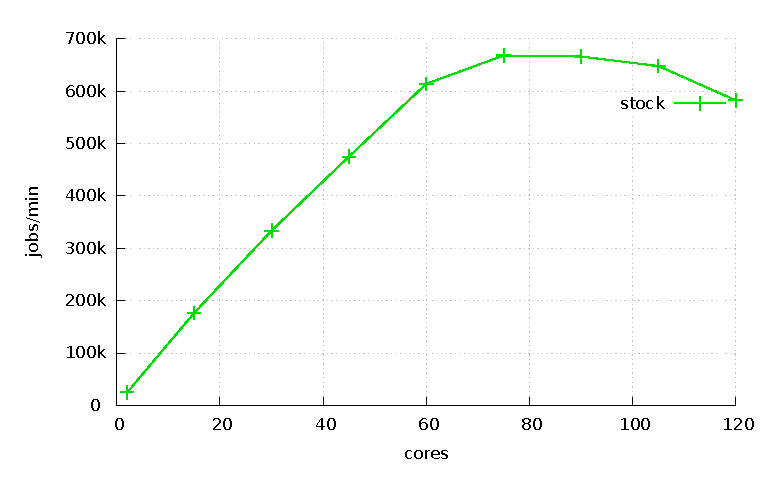
\includegraphics[width=0.8\textwidth]{graph/aim7_default}
    \caption{AIM7-multiuser 성능 확장성}
  \label{fig:aim7_default}
\end{figure}

\begin{figure}[h]
    \centering
    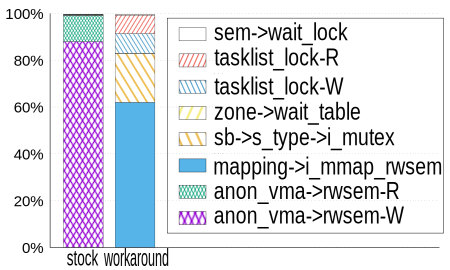
\includegraphics[width=0.8\textwidth]{graph/lockstat}
    \caption{120코어에서 락 때문에 기다리는 시간}
  \label{fig:aim7_default}
\end{figure}

운영체제 커널의 병렬화(Parallelism)는 시스템 전체의 병렬화에서 가장 중요한 부분이다.
만약에 커널이 확장성이 없으면, 그 위에 동작하는 응용프로그램들도 역시 확장성이
없게 된다~\cite{Clements15SCR}~\cite{Boyd-WickizerCorey}.
우리는 이처럼 중요한 운영체제 커널 중 멀티코어에 최적화된 리눅스 커널의 확장성을 분석하기 위해 
AIM7-multiuser 벤치마크를 사용하였다.
AIM7은 최근에도 성능 확장성을 위해 연구 진영과 리눅스 커널 커뮤니티 진영에서 활발히 사용되고 있는 
벤치마크 중 하나이다~\cite{Bueso2015STP}~\cite{Bueso2014MCS}.
AIM7-multiuser 워크로드는 동시에 많은 프로세스를 생성하며 디스크 파일(Disk File) 연산, 가상 
메모리(Virtual Memory) 연산, 파이프(Pipe), I/O(Input/Output) 그리고 수학 연산과 함께 수행한다.
우리는 파일 시스템의 성능 확장성을 최소화하기 위해, \code{tempfs}(Linux temp file system)를 사용하였다.
실험 결과 75코어까지 확장성을 가지나, 그 이후에서는 확장성이 떨어져 완만한 그래프를 보이는 문제점을 가진다. 

%$$$$$$$$$$$$$$$$$$$$$$$$$$$$$$$$$$$$$$$$$$$$$$$$$$$$$$$$$$$$$$$$$$$$$$$$$$$$$$$$
% Paragraph: Lockstat로 분석 결과 설명 
%$$$$$$$$$$$$$$$$$$$$$$$$$$$$$$$$$$$$$$$$$$$$$$$$$$$$$$$$$$$$$$$$$$$$$$$$$$$$$$$$
우리는 성능 확장성의 근본적인 문제를 분석하기 위해, 리눅스의
\code{lock\_stat}~\cite{LOCKSTAT}를 이용하여 120코어 부분에 락 경합을 분석하였다.
\code{lock\_stat}는 리눅스 커널에 있는 락 프로파일러(Profiler)이며, 
락을 얻기 위해 스레드가 얼마나 대기하였는지에 대한 대기 시간을 결과로 보여준다.
AIM7 벤치마크를 동작 시키고 120코어에서 락 경합을 분석 해보면, 
그림 ~\ref{fig:aim7_default}과 같은 결과를 얻는다.
실험 결과 AIM7 벤치마크는 익명(Anonymous) VMA(Virtual Memory Address)에서 상당히 많은 쓰기 락 경합이
발생한다.
이것은 수 많은 \code{fork}에 의해 프로세스를 생성하면서 발생하는 락 경합 문제이다.
리눅스가 \code{fork(), exit(), mmap()}시스템 콜(System Call)을 사용할 때 페이지(Page) 정보를
업데이트를 하게 되는데, 이 때 역 페이지 매핑(Revsers Page Mapping)의 연산이 이루어지고, 
동시에 락에 의해 스레드들은 직렬화가 된다. 

 \begin{figure}[h]
    \centering
    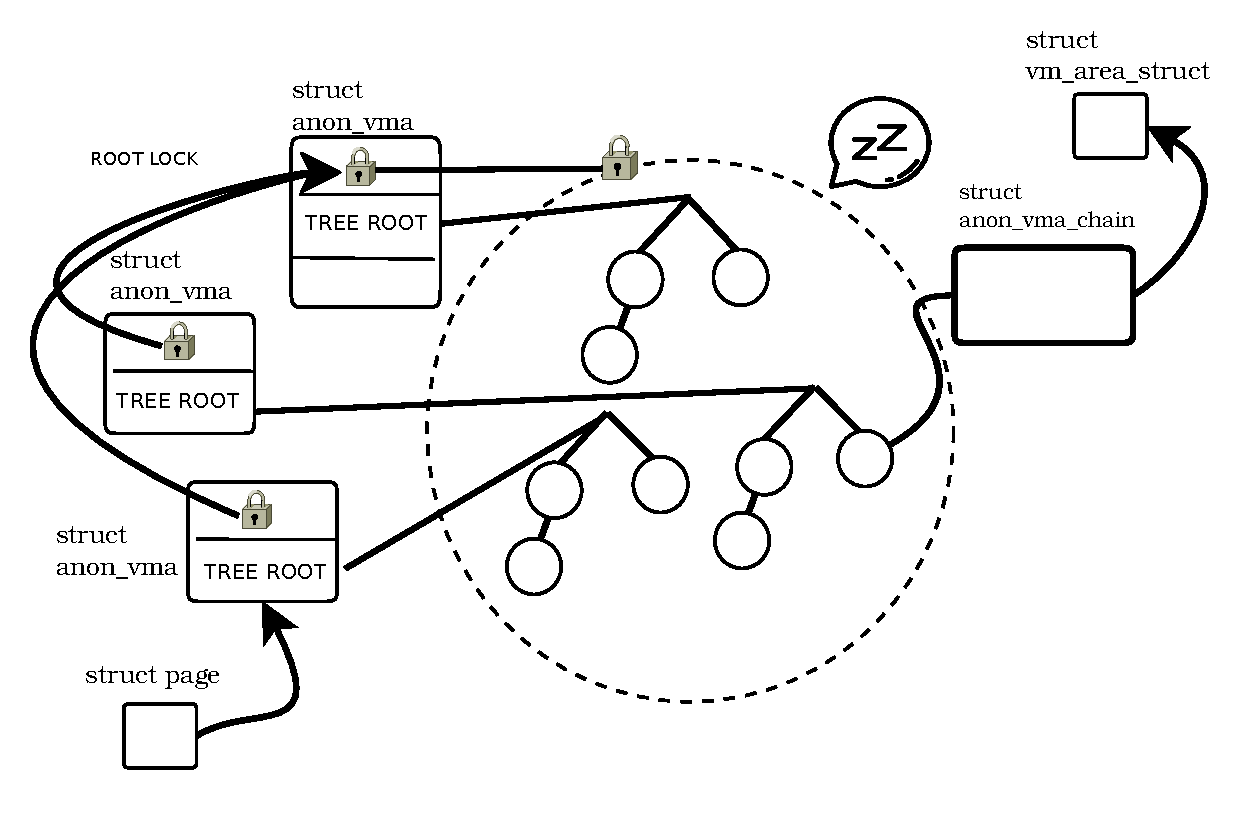
\includegraphics[width=0.8\textwidth]{fig/anon_vma_rmap}
    \caption{익명 역 매핑의 문제}
  \label{fig:anon_vma_rmap}
\end{figure}

다음으로 우리는 익명 역 매핑의 락 경합을 줄이기 위해, 임시로 \code{fork}에서 익명 역 매핑를 호출하는 부분과 
읽기 연산과 관련 있는 페이지 스왑(Page Swap)과 관련된 코드를 삭제하고, 다시 락 경합을 분석하였다. 
익명 역 매핑 관련 기능을 제거하면, 그 동안 상대적으로 가려졌던 파일 역 매핑에서 많은 락 경합이 발생되었다.
본 연구의 분석 결과 \code{fork}의 확장성 문제를 야기하는 것은 둘 중 하나가 아니라, 익명 역 매핑, 
파일 역 매핑 둘 모두 문제를 야기 한다고 볼 수 있다.

먼저 익명 역 매핑의 락 경합 문제는 그림~\ref{fig:anon_vma_rmap}이 보여준다.
그림은 물리적인 메모리 \code{struct page}에서 시작하여 그림의 오른쪽 상단의 
가상 메모리 영역인 \code{struct vm\_area\_struct}를 효율적으로 찾기 위한 과정을 보여준다. 
여기서 \code{struct anon\_vma\_chain}들은 모두 트리로 관리가 되며, 이 트리의 루트는
\code{struct anon\_vma}가 보관한다. 
모든 트리에 대한 연산은 \code{struct anon\_vma}가 가지고 있는 최상의 부모의 락에 의해 보호가 된다. 
따라서 \code{struct anon\_vma}의 모든 자식들은 모두 최상의 부모의 락 때문에 보호된다.
이것은 자식들의 트리 연산을 위해 접근하면 모두 블락에 걸리는 문제를 가진다. 
또한 파일 역 매핑의 락 경합 문제는 그림~\ref{fig:file_rmap_default}이 보이듯이 
익명 역 매핑 보다는 적지만, 트리에 접근하기 위해서는 \code{struct address\_space}의 락에 의해 
블락이 걸린다.

\begin{figure}[h]
    \centering
    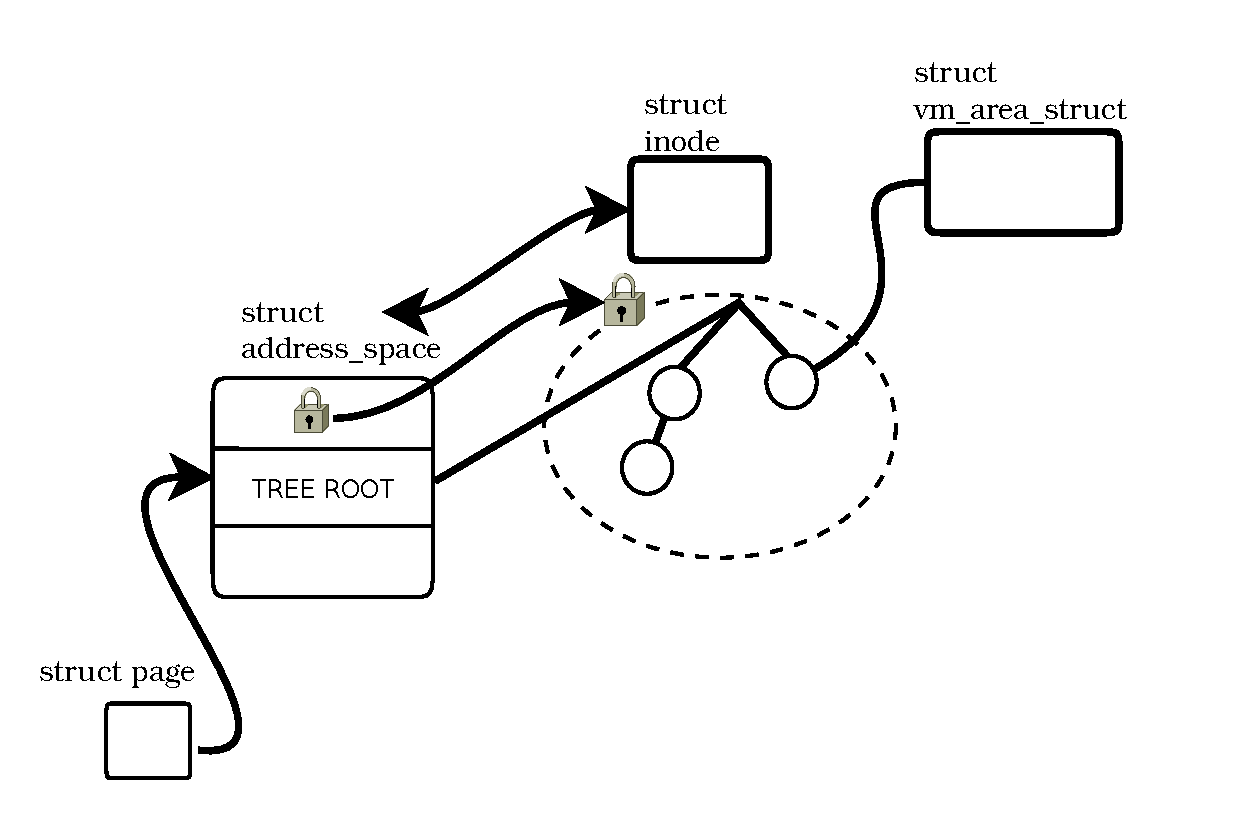
\includegraphics[width=0.8\textwidth]{fig/file_rmap_default}
    \caption{파일 역 매핑의 문제}
  \label{fig:file_rmap_default}
\end{figure}

%$$$$$$$$$$$$$$$$$$$$$$$$$$$$$$$$$$$$$$$$$$$$$$$$$$$$$$$$$$$$$$$$$$$$$$$$$$$$$$$$
% Paragraph : 리눅스 reverse page map의 write serialization 문제점
%$$$$$$$$$$$$$$$$$$$$$$$$$$$$$$$$$$$$$$$$$$$$$$$$$$$$$$$$$$$$$$$$$$$$$$$$$$$$$$$$
익명 역 페이지 매핑은 리눅스 커뮤니티에서 잘 알려진 락 경합 문제~\cite{Andi2011adding}이고, 
파일 페이지 역 매핑에 대한 락 경합 문제는 S. Boyd-Wickizer가 OpLog 논문을 통해 \code{fork}의 확장성 
문제의 중요한 원인으로 제시한 부분이다.
본 연구에서는 익명 역 매핑과 파일 역 매핑 두 가지 모두 개선해야지 \code{fork}의 성능 확장성이 
향상 된다는 것을 분석하였다. 

\begin{figure}[h]
    \centering
    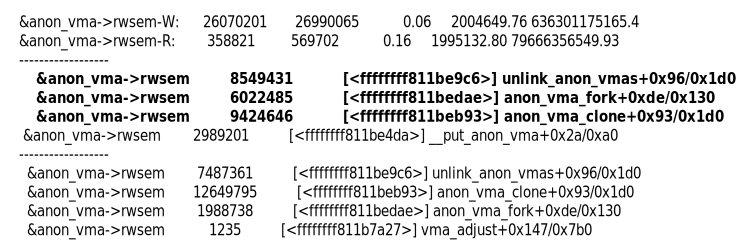
\includegraphics[width=0.8\textwidth]{fig/anon_vma_func}
    \caption{120코어에서의 lock\_stat 결과 분석}
  \label{fig:anon_vma_func}
\end{figure}

\begin{figure}[h]
    \centering
    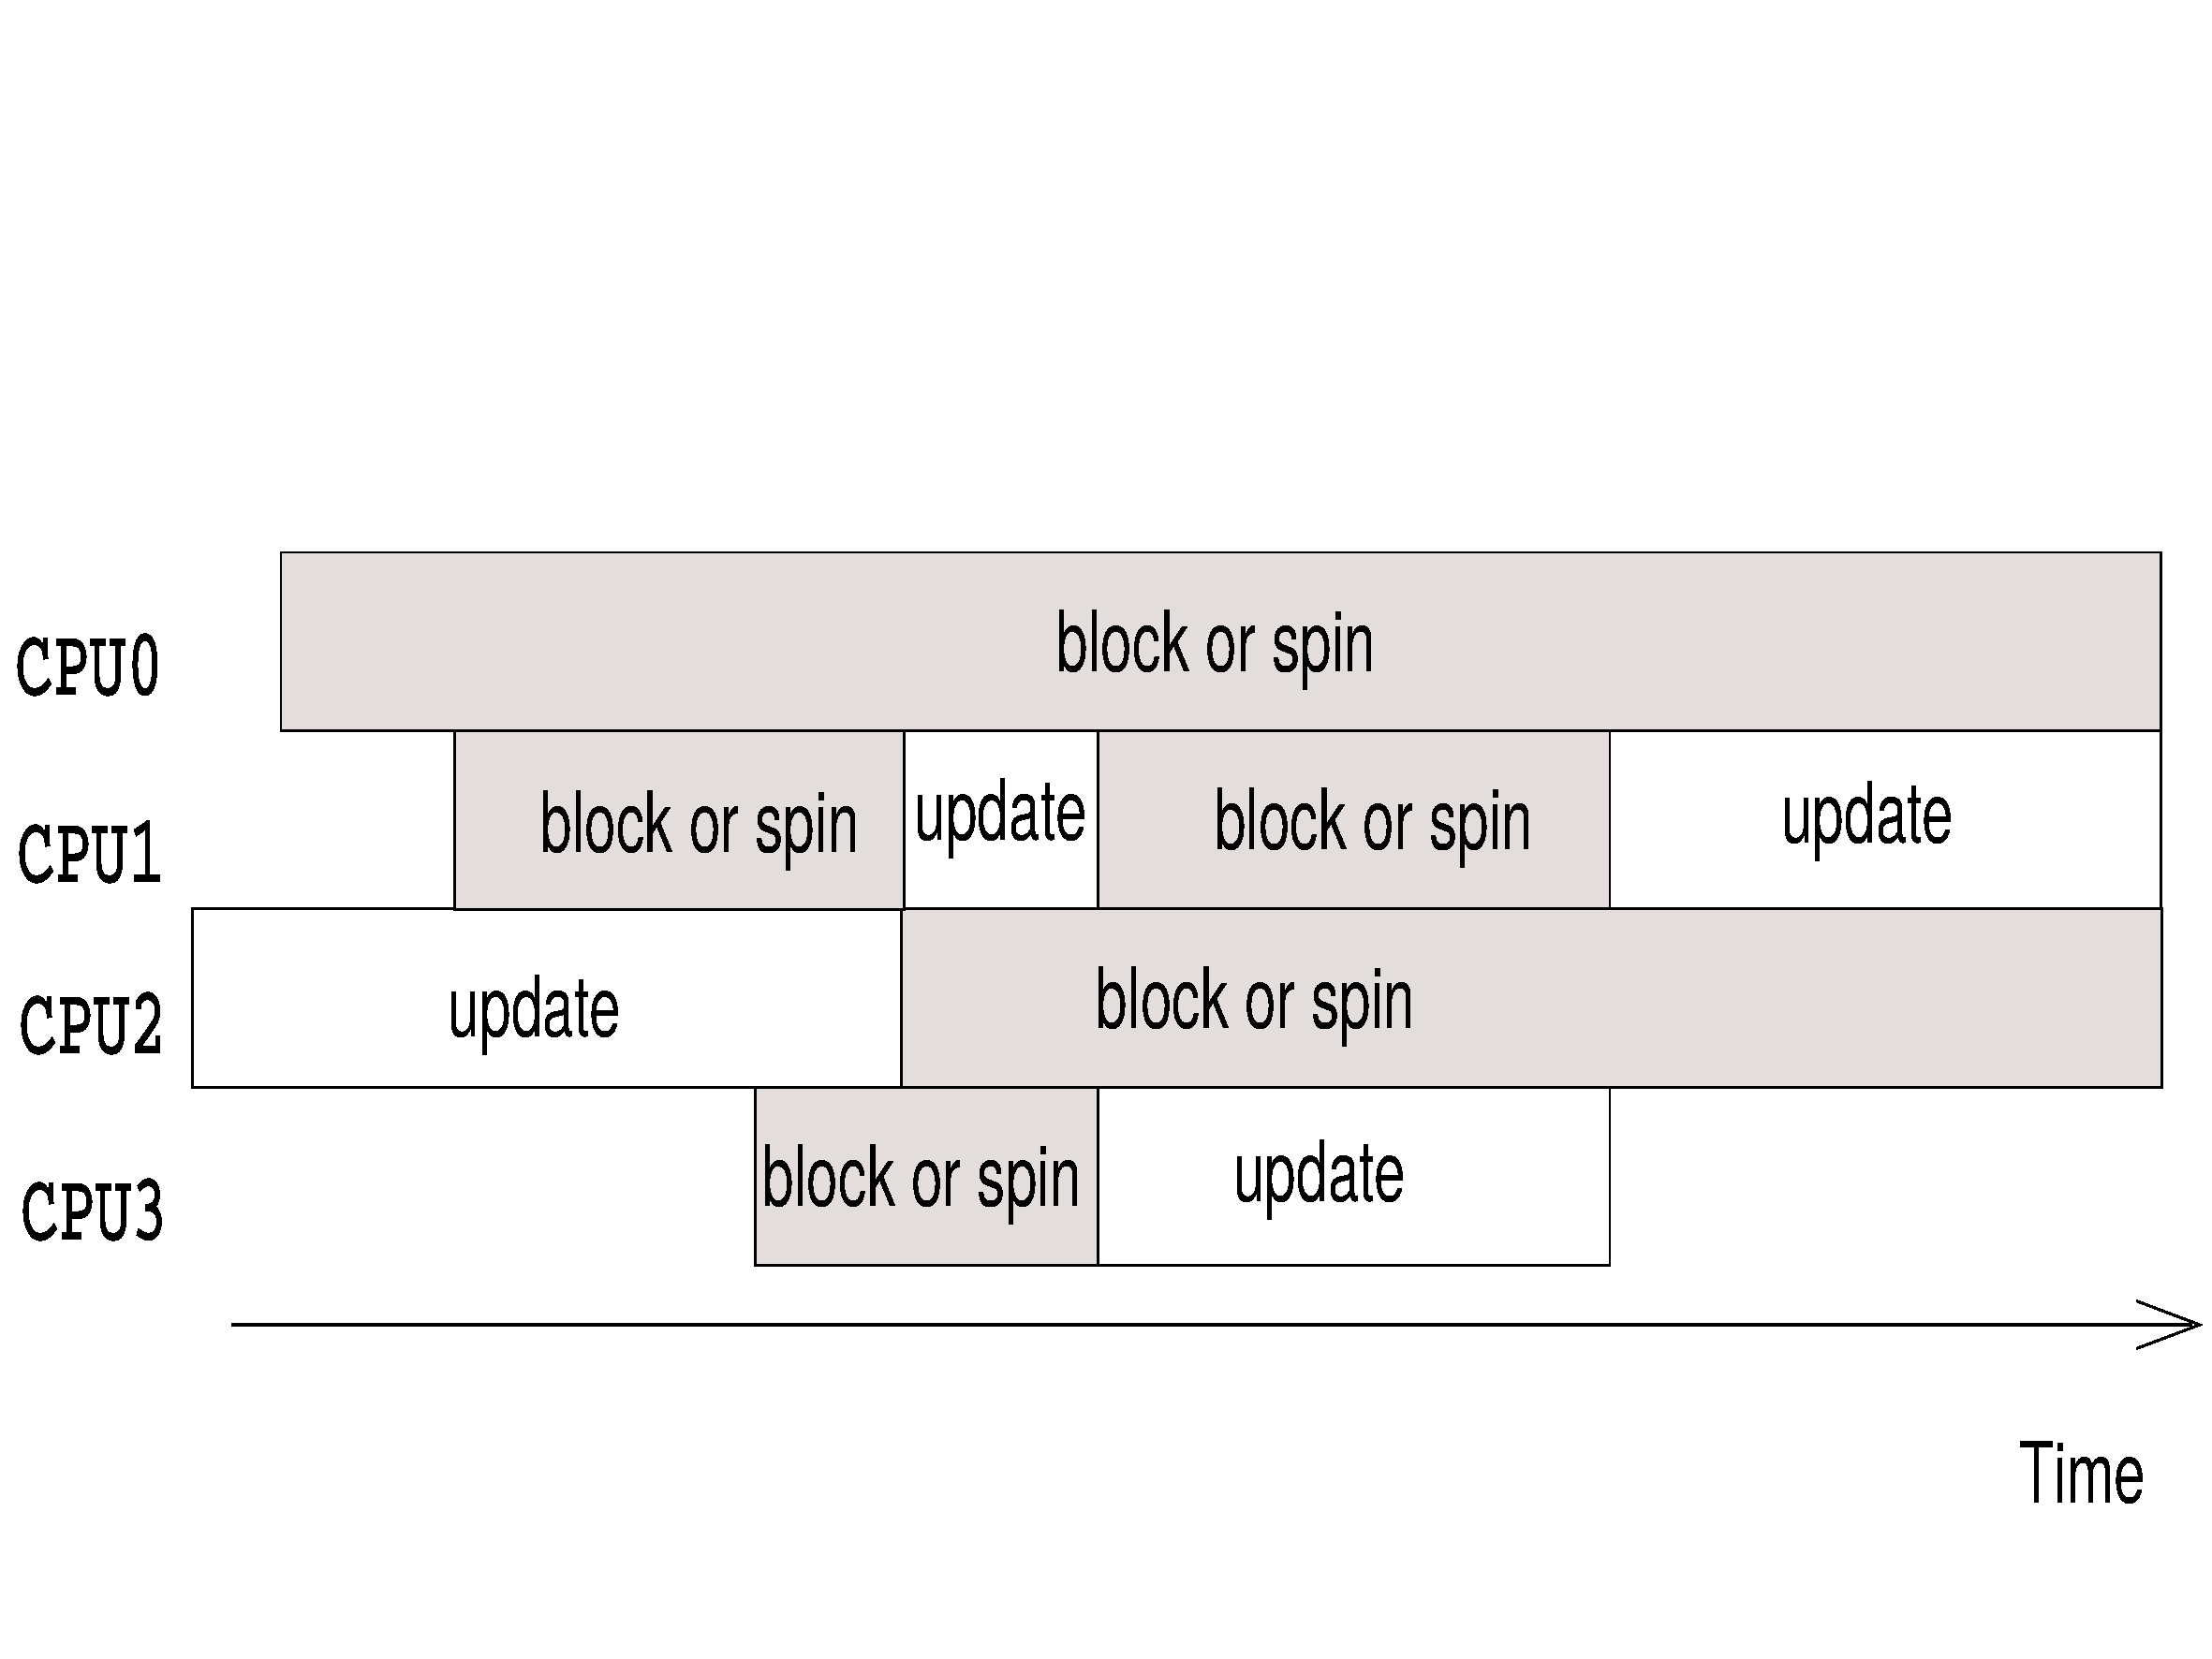
\includegraphics[width=0.8\textwidth]{fig/update}
    \caption{업데이트 직렬화의 문제}
    \label{fig:update}
\end{figure}

%$$$$$$$$$$$$$$$$$$$$$$$$$$$$$$$$$$$$$$$$$$$$$$$$$$$$$$$$$$$$$$$$$$$$$$$$$$$$$$$$
% Paragraph : update heavy한 상황에 대한 설명과 해결 방법에 대한 설명
%$$$$$$$$$$$$$$$$$$$$$$$$$$$$$$$$$$$$$$$$$$$$$$$$$$$$$$$$$$$$$$$$$$$$$$$$$$$$$$$$
락을 호출하는 함수들을 분석해보면 그림~\ref{fig:anon_vma_func}과 같다.
경합이 발생되는 함수(\code{unlink\_anon\_vma, anon\_vma\_fork, anon\_vma\_clone)}들의 
특징을 보면 대부분 자료구조 업데이트 연산을 수행하는 함수들이다. 
결국 높은 업데이트 비율이 때문에 락 경합이 많이 발생한 것이다.
업데이트 락 경합의 문제점은 그림~\ref{fig:update}와 같이 어떠한 동기화 기법을 사용해도 
결국 업데이트 연산에서는 직렬화가 된다는 것이다.

이처럼 높은 업데이트 비율 때문에 발생하는 업데이트 직렬화 문제를 해결하기 위해 그 동안 여러 방법이 
제안되었다. 
연구된 방법들은 논블락킹 알고리즘을 이용하는 
방식과 로그 기반 알고리즘을 사용하는 방법이 있다.
논블락킹 알고리즘들은 하드웨어 동기화 연산들을 활용하여
락과 같은 동기화 메커니즘 없이 업데이트와 읽기 연산을 수행하는 방법이다.
예를 들어, 논블락킹 알고리즘들은 업데이트 연산을 수행할 때, 업데이트를 원자적인 CAS(Compare And Swap) 
명령으로 전역 변수가 변경되었는지 확인한 후 수정하는 일을 수행한다.
만약 다른 스레드들에 의해 전역변수가 수정되었다면 CAS 연산은 실패되고, 업데이트 연산은 
처음 부터 다시 수행된다. 
결국 다른 스레드가 같은 메모리 주소의 내용을 변경을 안 할때까지 CAS를 이용해 반복 적으로 
확인하는 방법으로 동시적 업데이트를 보장한다. 
하지만 이러한 방법도 결국 공유 메모리 주소에 다수의 스레드가 CAS로 접근하여 병목 현상이 생긴다. 
이것은 결국 캐시 일관성 트래픽을 만든다~\cite{SilasBoydWickizerPth}.
최근에는 이처럼 캐시 일관성 트래픽 문제를 발생 시키는 연산을 줄인 로그 기반 방법들이 연구되고 있다.

%$$$$$$$$$$$$$$$$$$$$$$$$$$$$$$$$$$$$$$$$$$$$$$$$$$$$$$$$$$$$$$$$$$$$$$$$$$$$$$$$
%Paragraph : Log 기반의 알고리즘 대략적인 설명 
%$$$$$$$$$$$$$$$$$$$$$$$$$$$$$$$$$$$$$$$$$$$$$$$$$$$$$$$$$$$$$$$$$$$$$$$$$$$$$$$$
로그 기반 알고리즘은 업데이트 비율이 많은 자료구조에 적합한 알고리즘이다. 
로그 기반 알고리즘은 락을 피하기 위해 업데이트 연산이 발생하면, 자료구조의 업데이트 
연산(삽입 또는 삭제)을 함수 인자(Argument)와 함께 저장하고, 주기적 또는 읽기 연산이 
수행되기 전에 그 동안 저장된 로그를 수행하는 방법이다.
이러한 로그 기반 방법은 마치 CoW(Copy on Write)와 유사하다.
즉, 읽기 연산에 저장된 로그가 수행됨으로 읽기가 간헐적으로 수행되는 자료구조에 적합한 방법이다.

이처럼 업데이트 비율이 많은 자료구조를 위한 로그 기반 방법은 총 4가지의 장점을 가진다. 
첫째, 업데이트가 수행하는 시점 즉 로그를 저장하는 순간에는 락이 필요 없다. 
따라서 락 자체가 가지고 있는 캐시 일관성 오버헤드를 줄일 수 있다. 
둘째로, 저장된 순차적인 업데이트 명령을 하나의 코어에서 수행하기 때문에, 캐시 지역성이 높아진다.
셋째, 큰 수정 없이 기존 여러 자료구조(Tree, List)에 쉽게 적용할 수 있는 장점이 있다.
마지막으로 저장된 로그를 실제 수행하지 않고, 여러 가지 최적화 방법을 사용하여 적은 
명령으로 로그를 줄일 수 있다. 
LDU도 로그 기반 방법을 따른다. 그러므로 앞에서 설명한 로그 기반 방법의 장점을 모두 가짐과 동시에
업데이트 순간 삭제 가능한 로그를 지우는 최적화 방법으로 성능이 향상된다.


\chapter{로그 기반 동시적 업데이트 방법}
\section{Design}
\label{sec:ldu}

%$$$$$$$$$$$$$$$$$$$$$$$$$$$$$$$$$$$$$$$$$$$$$$$$$$$$$$$$$$$$$$$$$$$$$$$$$$$$$$$$
%Paragraph 1: LDU의 특징을 간단한 설명과 이번장에 대한 설명(LDU의 특징을 요약하여 설명)
%$$$$$$$$$$$$$$$$$$$$$$$$$$$$$$$$$$$$$$$$$$$$$$$$$$$$$$$$$$$$$$$$$$$$$$$$$$$$$$$$

The \LDU is a log-based concurrent update method to remove scalability
bottlenecks for the update-heavy data structure.
The \LDU further improves the performance scalability for update-heavy data structures
by eliminating the synchronized time-stamp management overhead from previous
research. One additional advantage of using the \LDU is that it reuses the log
slots already allocated and used by preceding operations.
%The previous research using the synchronized time-stamp counters method may incur
%time-stamp merging and ordering overhead.
%The \LDU can solve these sequential processing by using two techniques.
%The \LDU instantly removes operation logs at update time that requires time-stamp
%counter and reuses the garbage log instead of creating a new log
%thereby eliminating the synchronized time-stamp counter and cache communication
%bottleneck.
This section explains these algorithmic design aspects of the \LDU.

\subsection{Approach}


%$$$$$$$$$$$$$$$$$$$$$$$$$$$$$$$$$$$$$$$$$$$$$$$$$$$$$$$$$$$$$$$$$$$$$$$$$$$$$$$$
%Paragraph 2: timestamp가 필요한 이유 : time-sensitive update operation log.
%$$$$$$$$$$$$$$$$$$$$$$$$$$$$$$$$$$$$$$$$$$$$$$$$$$$$$$$$$$$$$$$$$$$$$$$$$$$$$$$$
The fundamental reason for requiring synchronized time-stamp counters is that some
operations need to be ordered.
For example, a process logs an insert operation to the per-core memory, then
it migrates to another core, and it logs a remove operation, which must eventually
execute after the insert operation~\cite{SilasBoydWickizerPth}.
%Thus, the synchronized time-stamp counters are needed.
To specifically explain a time-sensitive log, we use the symbol label used by
this paper~\cite{Clements15SCR}.
We describe insert as plus-circles $\oplus$, remove as minus-circles
$\ominus$ and object as color-circles \inv{2}{B}(object B). 
Color and vertical offset differentiate cpus.
For example
\begin{center}
$\oplus$\inv{1}{A}, $\oplus$\inv{2}{B}, $\oplus$\inv{3}{C},$\ominus$\inv{2}{A},
$\ominus$\inv{3}{C}, $\oplus$\inv{3}{A}, $\oplus$\inv{3}{C},$\ominus$\inv{1}{C}
\end{center}
consists of five insert operations, three remove operation, three cpus, and
three objects.
This example shows that $\oplus$\inv{1}{A} and $\ominus$\inv{2}{A},
time-sensitive logs, must be executed in chronological order.
The \LDU can eliminate this time-sensitive logs at update time;as a result, the synchronized time-stamp counters are eliminated.
One more important fact that these time-sensitive operation logs may be removed
by optimization phase.
For example, insert-remove operations or remove-insert operations, 
$\oplus$\inv{1}{A}$\ominus$\inv{2}{A}, $\oplus$\inv{3}{C}$\ominus$\inv{3}{C} 
and $\oplus$\inv{3}{C}$\ominus$\inv{1}{C}, are the cancelable operations before
a reader, so the remained operation logs, 
\begin{center}
 $\oplus$\inv{2}{B}, $\oplus$\inv{3}{A}
\end{center}
, are non-time-sensitive logs.
When update operations occur, the \LDU removes these time-sensitive logs using
the update-side removing technique.

%$$$$$$$$$$$$$$$$$$$$$$$$$$$$$$$$$$$$$$$$$$$$$$$$$$$$$$$$$$$$$$$$$$$$$$$$$$$$$$$$
%Paragraph 3:  time-sensitive update operation 삭제 방법: Update-side Abosrbing 
%$$$$$$$$$$$$$$$$$$$$$$$$$$$$$$$$$$$$$$$$$$$$$$$$$$$$$$$$$$$$$$$$$$$$$$$$$$$$$$$$

To remove the time-sensitive log, the \LDU uses the update-side removing scheme.
When insert-remove operations occur in terms of the same object, the scheme removes the insert-remove operations at update time.
The OpLog also optimizes by removing the existing operation rather than
adding the new one, but the OpLog can not remove log when a thread 
migrates other core, so it needs additional sequential processing during
the optimization phase.
The \LDU, however, has no problem with the migrating other core during logging
process because it uses the shared atomic swap operation in an individual object.

%$$$$$$$$$$$$$$$$$$$$$$$$$$$$$$$$$$$$$$$$$$$$$$$$$$$$$$$$$$$$$$$$$$$$$$$$$$$$$$$$
%Paragraph 5: 리눅스의 Update-side removing 수행 방법
%$$$$$$$$$$$$$$$$$$$$$$$$$$$$$$$$$$$$$$$$$$$$$$$$$$$$$$$$$$$$$$$$$$$$$$$$$$$$$$$$
The update-side removing logs scheme performs an atomic swap operation in an
individual object for shared memory systems.
This atomic swap operation allows update operations to atomically remove with the
previous cancelable log.
To achieve update-side removing log, 
first, add the mark field to the individual object
structure then use it as a status flag. 
For example, consider the insert-remove operation sequence at the same object.
The first insert operation marks the mark field and then it logs into the queue.
If the remove operation occur, the \LDU will not logs;it only changes the mark field.
When the reader applies logs, the \LDU applies the logs to the original data
structure in case of the true value of the mark field.
The benefit of this update-side removing scheme is twofold:not only it can
eliminate the time-sensitive operation but also it can cancel the previous
operation log in the queue.

%$$$$$$$$$$$$$$$$$$$$$$$$$$$$$$$$$$$$$$$$$$$$$$$$$$$$$$$$$$$$$$$$$$$$$$$$$$$$$$$$
%Paragraph 7: 또 최적화 방법 reusing garbage object : 
%$$$$$$$$$$$$$$$$$$$$$$$$$$$$$$$$$$$$$$$$$$$$$$$$$$$$$$$$$$$$$$$$$$$$$$$$$$$$$$$$

The second technique, called reusing garbage logs, reuses the garbage log
instead of creating a new log.
The garbage log is the log that has been already cancelled by 
using the update-side removing scheme,
but it still occupies a slot in the queue.
For example, consider the insert-remove-insert operations.
After the second remove operation, the log is remaining in the queue, but it has been
already cancelled by using update-side removing; hence {\it insert} mark field
is zero in the queue.
In this case, the third insert operation reuses the log in the queue instead of 
creating a new log using the atomic swap, so it can reduce not only the memory
overhead but also the queuing overhead.

%$$$$$$$$$$$$$$$$$$$$$$$$$$$$$$$$$$$$$$$$$$$$$$$$$$$$$$$$$$$$$$$$$$$$$$$$$$$$$$$$
%Paragraph 11: 중간에 한번씩 log를 flush
%$$$$$$$$$$$$$$$$$$$$$$$$$$$$$$$$$$$$$$$$$$$$$$$$$$$$$$$$$$$$$$$$$$$$$$$$$$$$$$$$
In addition to the update-side removing logs and the reusing garbage logs,
the \LDU uses the previous research's scheme that periodically applies the operation logs 
to reduce memory usage and to keep the log from growing without end.
This approach is similar with the method of previous research such as the OpLog's
batching updates and flat combining(FC)'s combiner thread.

%$$$$$$$$$$$$$$$$$$$$$$$$$$$$$$$$$$$$$$$$$$$$$$$$$$$$$$$$$$$$$$$$$$$$$$$$$$$$$$$$
%Paragraph 8: LDU의 로그는 두 종류의 queue에 저장할 수 있도록 지원
%$$$$$$$$$$$$$$$$$$$$$$$$$$$$$$$$$$$$$$$$$$$$$$$$$$$$$$$$$$$$$$$$$$$$$$$$$$$$$$$$
Furthermore, we design a log's queue using both the per-core and the global queue
to further support various data structures.
The per-core queue of the \LDU can remove CAS operations, which access global
head pointer. 
However, the per-core queue does not properly apply to all data structures since
it has some drawbacks.
The per-core queue has a memory overhead, and developers may need
an additional management code for per-core memory management(see section~\ref{sec:linux}).
To overcome these shortcomings, the \LDU also supports a global queue.
The global queue of the \LDU is simple and easy to apply, so it can easily use any
data structure.
Though global queue can not perfectly remove global CAS operations, it can
mitigate the cache communication overhead by using update-side removing
logs and by reusing garbage logs because it reduces the number of inserting the
queue(see section~\ref{sec:evaluation}-B).

%$$$$$$$$$$$$$$$$$$$$$$$$$$$$$$$$$$$$$$$$$$$$$$$$$$$$$$$$$$$$$$$$$$$$$$$$$$$$$$$$
%Paragraph 9: log를 저장하는 queue의 종류는 non-blocking queue를 사용
%$$$$$$$$$$$$$$$$$$$$$$$$$$$$$$$$$$$$$$$$$$$$$$$$$$$$$$$$$$$$$$$$$$$$$$$$$$$$$$$$
The \LDU uses the non-blocking queue regardless of the per-core queue or the
global queue since it can proceed without any lock.
Among non-blocking queues, the \LDU uses multiple producers and single consumer
based non-blocking queue thereby reducing the CAS operations.
This queue always inserts node where is a first pointer, so it can minimize
iteration loops because it causes another CAS operation.
In addition, this queue merely considers single consumer when it applies
the logs, so it does not need complex algorithms for the remove operation.
The queue uses atomic swap operation to acquire all operation logs.

\subsection{Example}
\begin{figure*}[h]
  \begin{center}
     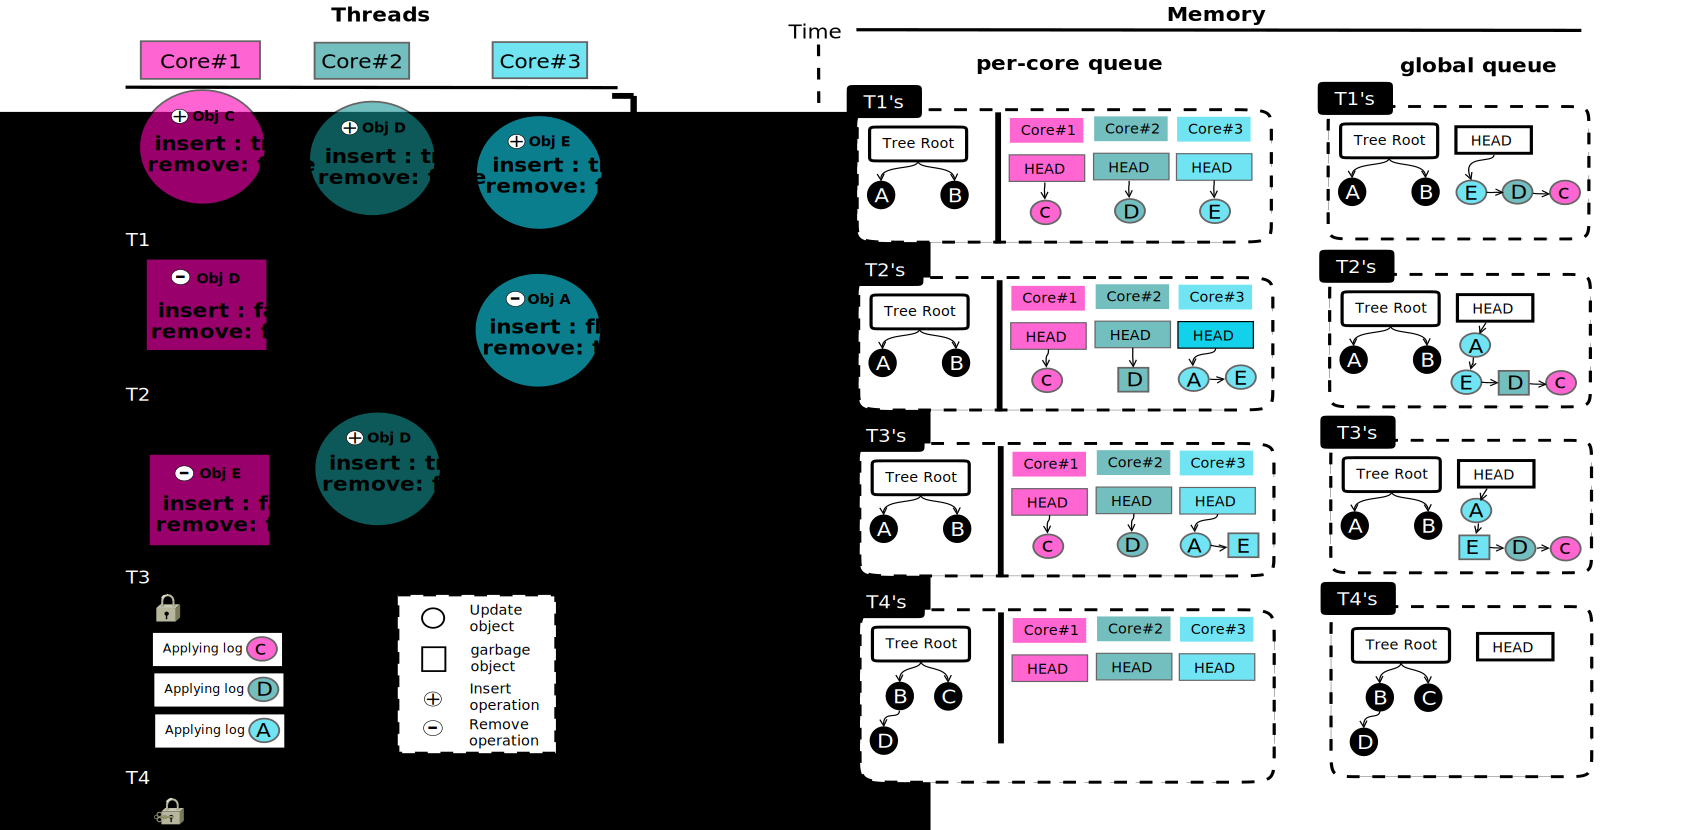
\includegraphics[width=1.0\textwidth,height=0.4\textheight]{fig/basic_gldu}
  \end{center}
  \caption{The \LDU example showing seven update operations(insert C, insert D ,
  insert E, remove D, insert A, insert D, and remove E) and one read
  operation. The execution flows from top to bottom.
  Memory represents original data structure and logging queue at T1, T2, T3 and T4,
  respectively. The initial tree data structure contains two object, A and B , and the queue is empty.
  The seven update operations concurrently execute without locks and a single
  reader executes with lock.}
  \label{fig:basic}
\end{figure*}

%$$$$$$$$$$$$$$$$$$$$$$$$$$$$$$$$$$$$$$$$$$$$$$$$$$$$$$$$$$$$$$$$$$$$$$$$$$$$$$$$
%Paragraph 1: Flowchart 구조 설명 
%$$$$$$$$$$$$$$$$$$$$$$$$$$$$$$$$$$$$$$$$$$$$$$$$$$$$$$$$$$$$$$$$$$$$$$$$$$$$$$$$

Figure \ref{fig:basic} shows an example of the \LDU with a per-core queue and
a global queue.
In order to explain the concurrent deferred update method for the update-heavy
data structure, we show how seven update operations can concurrently execute
without lock before the read operation.
The update operations sequence is
\begin{center}
$\oplus$\inv{1}{C}, $\oplus$\inv{2}{D}, $\oplus$\inv{3}{E},$\ominus$\inv{1}{D},
$\ominus$\inv{3}{A}, $\oplus$\inv{2}{D}, $\ominus$\inv{1}{E}. 
\end{center}.
To explain the \LDU, we use the previously used symbols with a new garbage symbol as
rectangle \res{1}{D}.
In this figure, execution flows from top to bottom.
The left side of figure shows cpu operations, and the right side of figure shows data structures
contents at a particular time in a memory.
Initially, the tree data structure contains \inv{0}{A} and \inv{0}{B}, and 
the queue is empty.

%$$$$$$$$$$$$$$$$$$$$$$$$$$$$$$$$$$$$$$$$$$$$$$$$$$$$$$$$$$$$$$$$$$$$$$$$$$$$$$$$
%Paragraph 2: Flowchart 그림 설명 
%$$$$$$$$$$$$$$$$$$$$$$$$$$$$$$$$$$$$$$$$$$$$$$$$$$$$$$$$$$$$$$$$$$$$$$$$$$$$$$$$
In the top of figure, \code{Core1}, \code{Core2} and \code{Core3} perform the
concurrent update operations, $\oplus$\inv{1}{C}, $\oplus$\inv{2}{D} and
$\oplus$\inv{3}{E}, without lock.
Since the \LDU uses non-blocking queue to save the operation logs, this step does not need
a update lock, so all threads can be executed in parallel without any lock contention.
At \code{T1}, the tree contains objects \inv{0}{A} and \inv{0}{B}. 
The per-core queue and the global queue contain $\oplus$\inv{1}{C}, $\oplus$\inv{2}{D} and
$\oplus$\inv{3}{E}, but the logs in the per-core queue are separated.

The next operations are $\ominus$\inv{1}{D} and $\ominus$\inv{3}{A}.
When the $\ominus$\inv{1}{D} operation is executed, the \LDU atomically changes 
the mark field in the object instead of inserting the queue.
Then, $\ominus$\inv{3}{A} inserts the queue because it is a new operation log.
At \code{T2}, the per-core queue and the global queue contain 
$\oplus$\inv{1}{C}, $\oplus$\res{2}{D}, $\oplus$\inv{3}{E} and
$\ominus$\inv{3}{A}.
The insert mark field in the object \res{2}{D} is false, called a garbage object, 
has remained in the queue, but it was already canceled 
by update-side removing logs.

The last operations are $\oplus$\inv{2}{D}, $\ominus$\inv{1}{E}.
The \LDU reuses the log in the queue instead of 
creating a new log using atomic swap.
Thus, the object \res{2}{D} changes \inv{2}{D}, and then the object \inv{3}{E} 
changes \res{3}{E} by performing the update-side removing logs scheme.
At \code{T3}, per-core queue contains
$\oplus$\inv{1}{C}, $\oplus$\inv{2}{D}, $\ominus$\inv{3}{A} 
and $\oplus$\res{3}{E}.

Before the read function, it need to lock the original tree lock using the
exclusive lock in order to protect the tree operations.
The \LDU migrates from queue to tree, each of which is the marked object.
Thus, $\oplus$\inv{1}{C}, $\oplus$\inv{2}{D} and $\ominus$\inv{3}{A} are
migrated except for the $\oplus$\res{3}{E} a garbage log.
At T5, the tree contains \inv{0}{B}, \inv{0}{C} and
\inv{0}{D}, so finally, the reader can read eventually consistent data.


\begin{figure*}[h]
\begin{center}
\inputminted[linenos,fontsize=\footnotesize, tabsize=2]{c}{src/ldu_logical_a.c}
\end{center}
\caption{The \LDU concurrent insert algorithm.  This logging may be called by
original update functions without locks. The concurrent update functions are
divided into three phase.}
\label{fig:gldulogicalupdate}
\end{figure*}


\begin{figure*}[h]
\begin{center}
\inputminted[linenos,fontsize=\footnotesize, tabsize=2]{c}{src/ldu_logical_b.c}
\end{center}
\caption{The \LDU concurrent remove algorithm.}
\label{fig:gldulogicalupdate}
\end{figure*}


\subsection{The Algorithm and Correctness}

This section shows skeleton of an algorithm.
We exclude the log's queue and the \LDU's detailed data structures for
exposition simplicity.

\subsubsection{inserting logs}
%$$$$$$$$$$$$$$$$$$$$$$$$$$$$$$$$$$$$$$$$$$$$$$$$$$$$$$$$$$$$$$$$$$$$$$$$$$$$$$$$
%Paragraph 1:LDU Concurrent Updates 알고리즘 코드 및 설명 
%$$$$$$$$$$$$$$$$$$$$$$$$$$$$$$$$$$$$$$$$$$$$$$$$$$$$$$$$$$$$$$$$$$$$$$$$$$$$$$$$
Figure \ref{fig:gldulogicalupdate} shows concurrent update functions.
The concurrent update functions are divided into three phase.
The first phase checks this object to see whether or not the
object is a cancelable object(Line 4, 20).
When this code is executed, the \code{synchronize} function can
be invoked by a reader or a periodic timer, so phase 1 needs the atomic operation.
If the corresponding mark field is true, then its mark field is changed to false.
In phase 2 checks this log to see weather or not has already inserted in
the queue(Line 8, 24).
If so, because mark field is marked(Line 6, 22), this function directly returns
true.
In the last phase, the operation log inserts the non-blocking queue
when the operation log is the first used log(Line 12, 28).

%$$$$$$$$$$$$$$$$$$$$$$$$$$$$$$$$$$$$$$$$$$$$$$$$$$$$$$$$$$$$$$$$$$$$$$$$$$$$$$$$
%Paragraph 4: 리눅스의 update operation의 특징을 이용한 Update-side Abosrbing 
%$$$$$$$$$$$$$$$$$$$$$$$$$$$$$$$$$$$$$$$$$$$$$$$$$$$$$$$$$$$$$$$$$$$$$$$$$$$$$$$$
This algorithm is correct because Linux kernel has a unique update
operations sequence.
For example, if an insert operation occur, then next operation must be a remove
operation at the same object because the kernel's update function
is separated from search, alloc and free functions.
The remove-remove or insert-insert operation in Linux kernel is
forbidden: if remove-remove operation occur, the second remove operation may
encounter a crash because this object can be concurrently freed after the first remove
operation, so we check the corresponding mark field(Line 5, 21).

\subsubsection{applying logs}

\begin{figure*}[h]
\begin{center}
\inputminted[linenos,fontsize=\footnotesize, tabsize=2]{c}{src/ldu_physical.c}
\end{center}
%\rule{\columnwidth}{0.5pt}
%\vspace{-\baselineskip}
\caption{The \LDU applying logs algorithm. The \code{synchronize\_ldu} may be
 called by a reader or a timer handler and converts logs to original data structure
 traversing the log's queue.}
\label{fig:glduphysicalupdate}
\end{figure*}


%$$$$$$$$$$$$$$$$$$$$$$$$$$$$$$$$$$$$$$$$$$$$$$$$$$$$$$$$$$$$$$$$$$$$$$$$$$$$$$$$
%Paragraph 2:LDU Deferred Updates 알고리즘 코드 및 설명 
%$$$$$$$$$$$$$$$$$$$$$$$$$$$$$$$$$$$$$$$$$$$$$$$$$$$$$$$$$$$$$$$$$$$$$$$$$$$$$$$$

Figure \ref{fig:glduphysicalupdate} shows deferred update function, which
applies the operation logs.
The \code{synchronize} function is invoked before the read, or it can be
periodically invoked by the timer handler because of preventing the continuous
growing the logs.
Before the execution of the \code{synchronize} function, it has been locked by using
the object lock, so this function proceed with a single consumer thread
in a way similar to the OpLog's batching updates and FC's combiner thread.
First, the \code{synchronize} function acquires queue's head pointer by using atomic swap
operation(Line 3).
Because the \LDU periodically applies the logs queue, the \LDU update operations may 
concurrently execute with the \code{synchronize} function.
Thus, before the applying original data structure, the mark field is
set to false(Line 8, 9).
The used flag for the garbage log is set to false indicating that the queue
does not contain this object(Line 10).
The \code{synchronize} function
once again checks(Line 12, 13) to see whether the mark field
is changed between the applying logs(Line 8) and clearing garbage bit(Line 10).

\section{Applying Linux kernel}
\label{sec:linux}

%\subsection{Reverse mapping}

%$$$$$$$$$$$$$$$$$$$$$$$$$$$$$$$$$$$$$$$$$$$$$$$$$$$$$$$$$$$$$$$$$$$$$$$$$$$$$$$$
%Paragraph 1: Linux의 reverse mapping에 대한 자세한 설명 
%$$$$$$$$$$$$$$$$$$$$$$$$$$$$$$$$$$$$$$$$$$$$$$$$$$$$$$$$$$$$$$$$$$$$$$$$$$$$$$$$

This section shows how to apply the \LDU to the complex Linux
virtual memory system 
to solve the update serialization problem;it deals with more practical one.

The Linux reverse page mapping(rmap), a kernel memory management mechanism, consists
of anonymous rmap and file rmap, are a update-heavy data structure.
These two rmaps maintain virtual address(VMAs) to translate physical
addresses to virtual address~\cite{Dave2004OLSRMAP}, and the rmaps are a shared global resource between processes.
These global resource of rmap are managed by using a interval tree.
To protect these shared tree, Linux kernel uses the reader-writer semaphore, and simultaneous creation of many processes becomes bottlenecks because
not only the rmap's update operations can not run
in parallel but also update's lock brings about the cache invalidation traffic.
On the contrary, the rmap rarely reads the interval tree when it swaps a physical page
out to disk, migrates other cpu, or truncates a file.
%In brief, the Linux rmaps are a update-heavy data structure. 

\subsection{Anonymous mapping}

\begin{figure}[tb]
  \begin{center}
     \includegraphics[width=1\textwidth,height=1\textheight,keepaspectratio]{fig/anon_vma}
  \end{center}
  \caption{An example of applying the \LDU to anonymous reverse mapping.
  When a process simultaneously spawns, the root lock leads to a scalability bottleneck. 
  The log's queue is added into the per-core memory or the
  global head object(\code{struct anon\_vma})}
  \label{fig:anonvmaramp}
\end{figure}

%$$$$$$$$$$$$$$$$$$$$$$$$$$$$$$$$$$$$$$$$$$$$$$$$$$$$$$$$$$$$$$$$$$$$$$$$$$$$$$$$
%Paragraph 1: linux의 anon vma의 공유된 구조에 대한 설명
%$$$$$$$$$$$$$$$$$$$$$$$$$$$$$$$$$$$$$$$$$$$$$$$$$$$$$$$$$$$$$$$$$$$$$$$$$$$$$$$$
Figure \ref{fig:anonvmaramp} shows the anonymous rmap data structure.
When a process spawns, the parent's anonymous vma chain(AVC) are copied
to a child, and then a new anonymous vma(\code{struct anon\_vma}) is created.
%, indicating the child's AVCs, 
When a process simultaneously spawns, the more complex
anonymous rmap data structures are created;the anonymous ramp is one of the complex data
structure in Linux kernel~\cite{CorbetLWNANON}.
The anonymous rmap uses the root lock since the AVCs are shared with child processes, so this root lock causes a lock contention problem~\cite{Andi2011adding}.

%$$$$$$$$$$$$$$$$$$$$$$$$$$$$$$$$$$$$$$$$$$$$$$$$$$$$$$$$$$$$$$$$$$$$$$$$$$$$$$$$
%Paragraph 2: anon vma에 ldu 적용한 방법에 대한 설명 
%$$$$$$$$$$$$$$$$$$$$$$$$$$$$$$$$$$$$$$$$$$$$$$$$$$$$$$$$$$$$$$$$$$$$$$$$$$$$$$$$
To eliminate this lock contention problem, we add the insert and
remove mark field in the individual object(\code{struct anon\_vma}),
and then we implement the update-side removing logs scheme.
Understanding the log's position of queue header is important.
As noted earlier, since the anonymous rmap uses the root lock, the per-core queue version of
the LDU logs into a per-core memory with root information, or the global
queue logs into a root data structure(\code{struct anon\_vma}).
Consequently, the \LDU does not largely modify the original data
structure, which shows why the \LDU is a lightweight method.

\subsection{File mapping}

\begin{figure}[tb]
  \begin{center}
     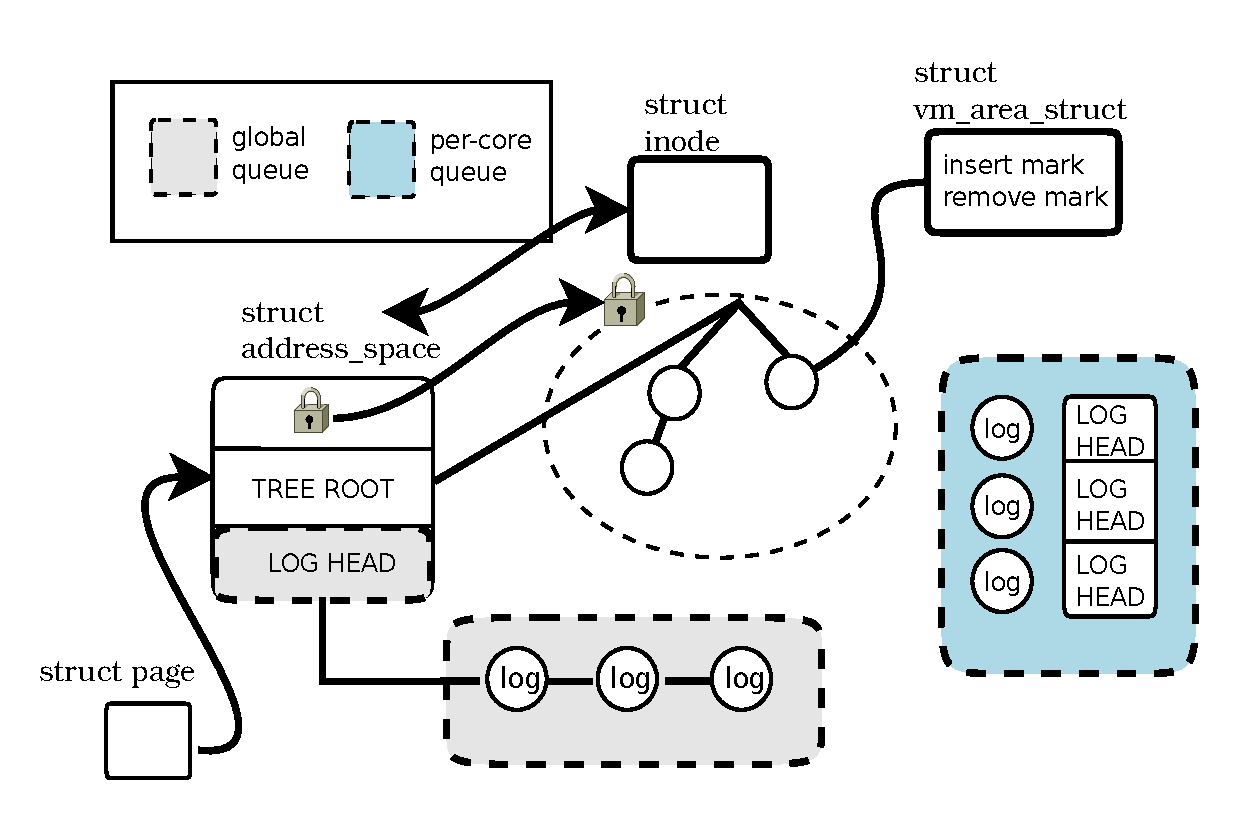
\includegraphics[width=1\textwidth,height=1\textheight,keepaspectratio]{fig/file_rmap}
  \end{center}
  \caption{An example of applying the \LDU to file reverse mapping. 
  The file rmap can be serialized at updating VMAs into the interval tree.
  The log's queue is added into the per-core memory or the
  global head object(\code{struct address\_space})}
  \label{fig:fileramp}
\end{figure}

%$$$$$$$$$$$$$$$$$$$$$$$$$$$$$$$$$$$$$$$$$$$$$$$$$$$$$$$$$$$$$$$$$$$$$$$$$$$$$$$$
%Paragraph 1: linux의 file mapped page reverse mapping의 구조에 대한 설명
%$$$$$$$$$$$$$$$$$$$$$$$$$$$$$$$$$$$$$$$$$$$$$$$$$$$$$$$$$$$$$$$$$$$$$$$$$$$$$$$$
Figure \ref{fig:fileramp} shows the rmap for file.
In order to translate physical addresses to virtual address, the page(\code{struct page})
indicates the address space object(\code{struct address\_space}), and
the address space object manages the VMAs by using the
interval tree.
This interval tree is a shared resource between processes.
%, so Linux kernel uses the reader-writer semaphore to protect the tree.
Because the system calls such as \code{fork()}, \code{exit()} and
\code{mmap()} entail concurrent updating VMAs into the shared resource.
when the processes simultaneously invoke these system calls, the
file rmap can be serialized at the update operations.

%$$$$$$$$$$$$$$$$$$$$$$$$$$$$$$$$$$$$$$$$$$$$$$$$$$$$$$$$$$$$$$$$$$$$$$$$$$$$$$$$
%Paragraph 2: file mapping에 ldu 적용한 방법에 대한 설명 
%$$$$$$$$$$$$$$$$$$$$$$$$$$$$$$$$$$$$$$$$$$$$$$$$$$$$$$$$$$$$$$$$$$$$$$$$$$$$$$$$
The \LDU can easily be applied to the file ramp data structure.
For instance, to use the \LDU, a developer adds log's queue header into the per-core
memory or into the original data structure(\code{struct address\_space}), and
then adds mark field to the individual object(\code{struct vm\_area\_struct}).
Then, the developer modifies update function to logging function without a lock.
Finally, the developer creates \code{synchronize} function and calls
the \code{synchronize} function before the read.
%the mark field adds to the individual object(\code{struct
%vm\_area\_struct}), and then the log's queue is added into the per-core
%memory or the global head object(\code{struct address\_space}).

This figure clearly shows why the \LDU additionally supports the
global queue because it is a simpler and easier scheme because the log's head
pointer is located in the interval tree's data structure.
On the other hand, the
per-core queue may need an additional per-core queue management scheme due
to the its isolated memory location.

\subsection{Detail Implementation}
%$$$$$$$$$$$$$$$$$$$$$$$$$$$$$$$$$$$$$$$$$$$$$$$$$$$$$$$$$$$$$$$$$$$$$$$$$$$$$$$$
%Paragraph 2: per-core queue 구현에 대한 설명 
%$$$$$$$$$$$$$$$$$$$$$$$$$$$$$$$$$$$$$$$$$$$$$$$$$$$$$$$$$$$$$$$$$$$$$$$$$$$$$$$$
Because the log's head pointer for the per-core queue is
separated with the original data structure, the implementation of
per-core queue uses 
a per-core hash table method that can allow each object to distinguish.
The per-core hash table implemented as a direct-mapped cache, which one
bucket only has an object because recently used objects will be in the hash
table in a way similar to the OpLog's per-core hash table.
When this hash table is met a hash conflict, the \LDU evicts the object in the
hash slot.
Moreover, this method reduces additional tasks of programmers because it can
minimize code modifications and does not need an additional lock.
The per-core hash table, however, incurs a hash conflict overhead.
This method is useful when a number of the root objects are infrequently created like the 
file rmap(\code{struct address\_space}).
On the other hand, since the anonymous rmap severely creates many
root objects(\code{struct anon\_vma}), it causes a hash conflict overhead.
Therefore, in the case of the anonymous ramp, we did not distinguish object
headers, but it needs additional tasks with global lock.

%$$$$$$$$$$$$$$$$$$$$$$$$$$$$$$$$$$$$$$$$$$$$$$$$$$$$$$$$$$$$$$$$$$$$$$$$$$$$$$$$
%Paragraph 1: 커널 버전 및 코드 분량, 테스트에 대한 설명
%$$$$$$$$$$$$$$$$$$$$$$$$$$$$$$$$$$$$$$$$$$$$$$$$$$$$$$$$$$$$$$$$$$$$$$$$$$$$$$$$
We have implemented the new deferred update algorithm in Linux 4.5-rc6 kernel,
and our modified Linux is available as open source. 
%The version of global queue modified code is xx that less complex, but per-core
%queue the modified code is xx-xx.
The implementation is stable enough and has passed the testing
related with virtual memory, scheduler,
and file in the Linux Test Project~\cite{LTP}.

\newpage

\section{평가}
\label{sec:evaluation}
\begin{figure}[h!]
  \begin{center}
    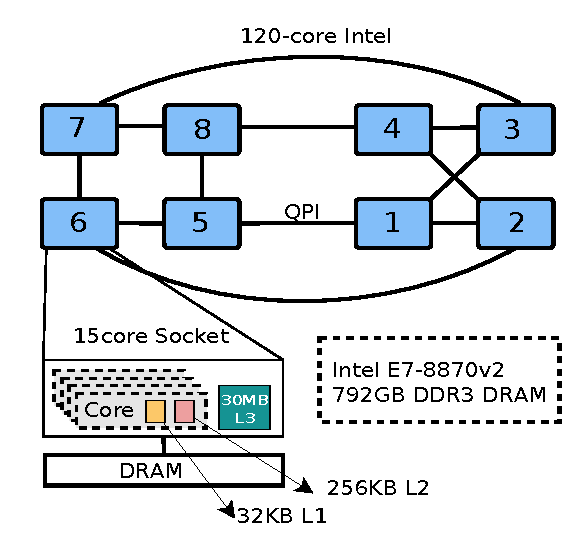
\includegraphics[scale=0.8]{fig/xeon}
  \end{center}
  \caption{실험 환경.}
  \label{fig:xeon}
\end{figure}
 
 \begin{figure}[h]
    \centering
    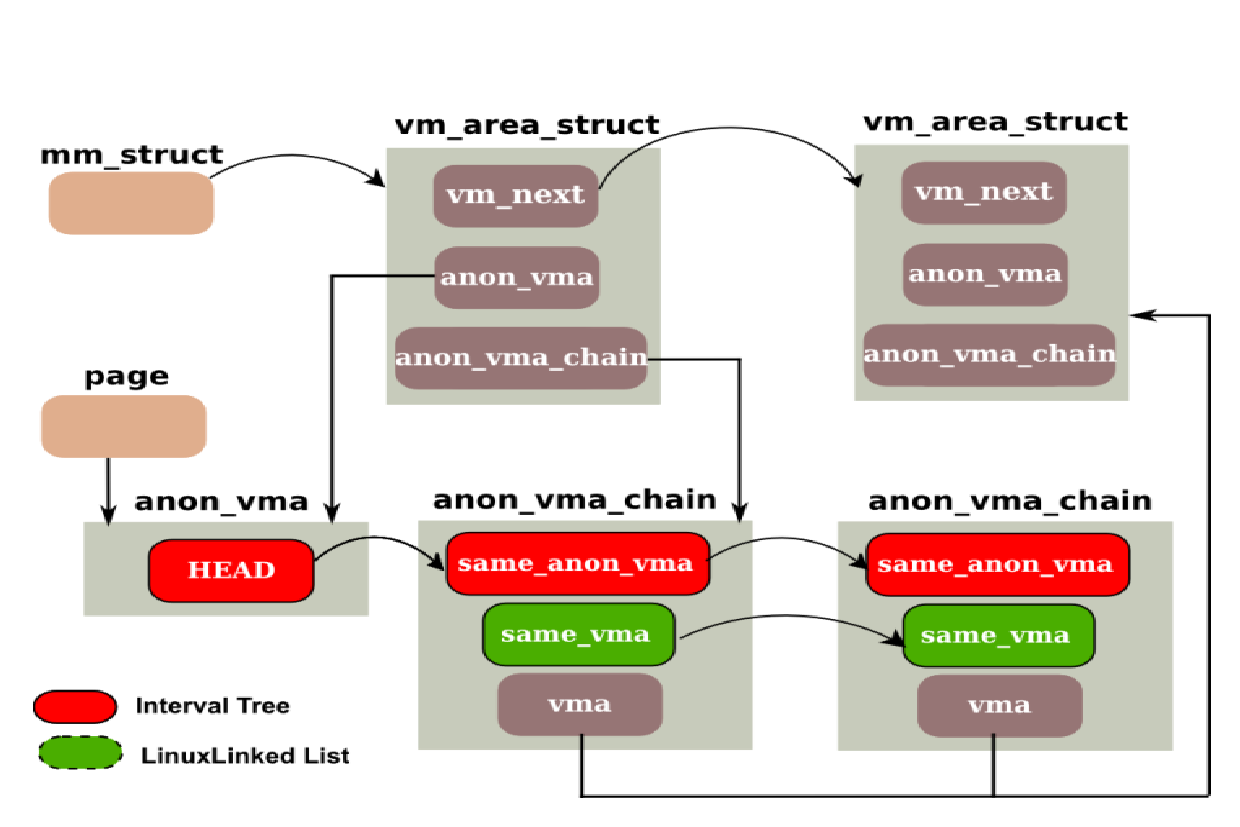
\includegraphics[width=0.8\textwidth]{fig/lockfree}
    \caption{lockfree 리스트로 변경하기 전 자료구조}
  \label{fig:lockfree}
\end{figure}
 
 \begin{figure}[h]
    \centering
    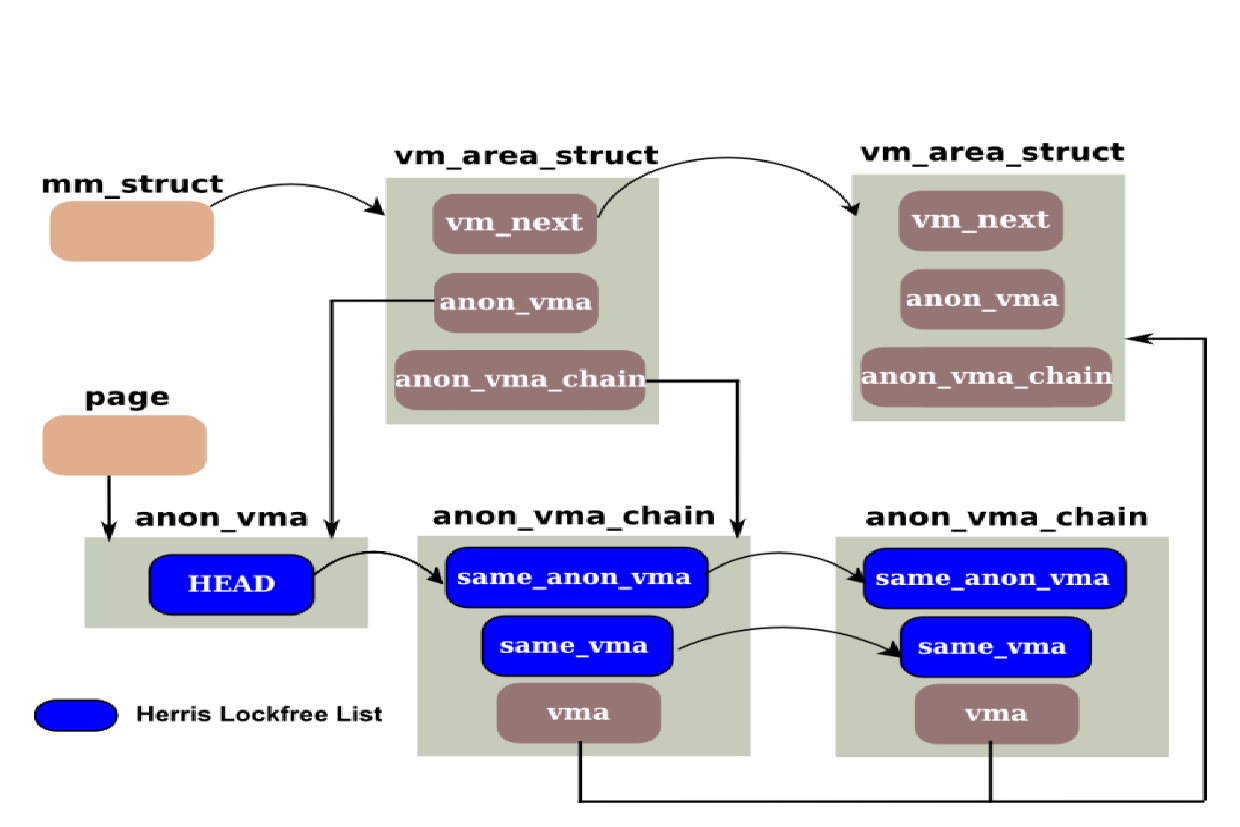
\includegraphics[width=0.8\textwidth]{fig/lockfree_2}
    \caption{lockfree 리스트로 변경 후 자료구조}
  \label{fig:lockfree_2}
\end{figure}

\subsection{실험 환경}

%$$$$$$$$$$$$$$$$$$$$$$$$$$$$$$$$$$$$$$$$$$$$$$$$$$$$$$$$$$$$$$$$$$$$$$$$$$$$$$$$
%Paragraph 1: 무엇을 평가 했는지에 대한 설명 
%$$$$$$$$$$$$$$$$$$$$$$$$$$$$$$$$$$$$$$$$$$$$$$$$$$$$$$$$$$$$$$$$$$$$$$$$$$$$$$$$
우리가 제안한 LDU 기법에 대해서 평가를 하기 위해, 우리는 리눅스 커널에 LDU를 적용하여 비교하였다.
비교 대상으로는 수정하지 않은 리눅스 커널과 Harris의 \code{lock-free} 리스트~\cite{Harris2001Lockfree}를 
구현하여 비교 실험을 하였다.
Harris 알고리즘을 사용한 이유는 논블락킹 알고리즘 중에서 대표하는 알고리즘이기 때문이다. 
Harris의 링크드 리스트의 기본적인 알고리즘은
\textit{sysnchrobench}~\cite{Gramoli2015Synchrobench}와
\textit{ASCYLIB}~\cite{David2015ASYNCHRONIZED}에서 구현된 내용을 이용했으며, 우리는 Harris 링크드
리스트를 리눅스 커널에 맞게 수정하여 적용하였다.
Harris 링크드 리스트의 적용을 예를 들어 설명하면 그림~\ref{fig:lockfree}과 같이 
\code{anon\_vma\_chain}의 내부 변수 중 \code{same\_anon\_vma}는 인터벌 트리로 되어 있고, 
\code{same\_vma}는 리눅스의 링크드 리스트로 되어 있다. 
두 자료구조를 논블락킹 링크드 리스트 중 하나인 Harris 링크드 리스트로 수정하여 구현을 하였다.

%$$$$$$$$$$$$$$$$$$$$$$$$$$$$$$$$$$$$$$$$$$$$$$$$$$$$$$$$$$$$$$$$$$$$$$$$$$$$$$$$
%Paragraph 3: 운영체제 및 커널 버전 설명
%$$$$$$$$$$$$$$$$$$$$$$$$$$$$$$$$$$$$$$$$$$$$$$$$$$$$$$$$$$$$$$$$$$$$$$$$$$$$$$$$
실험을 위해 사용한 하드웨어는 8소켓으로 구성된 120코어 시스템을 사용했으며,
각각의 코어는 인텔 E7-8870 chips(15 cores per socket)을 가진다.
메모리는 792기가 바이트 DDR3 DRAM을 사용하였다.
그림~\ref{fig:xeon}은 우리가 사용한 시스템을 보여준다.

%$$$$$$$$$$$$$$$$$$$$$$$$$$$$$$$$$$$$$$$$$$$$$$$$$$$$$$$$$$$$$$$$$$$$$$$$$$$$$$$$
%Paragraph 2-1: Harris Lock free list 구현 내용에 대한 설명 
%$$$$$$$$$$$$$$$$$$$$$$$$$$$$$$$$$$$$$$$$$$$$$$$$$$$$$$$$$$$$$$$$$$$$$$$$$$$$$$$$

%$$$$$$$$$$$$$$$$$$$$$$$$$$$$$$$$$$$$$$$$$$$$$$$$$$$$$$$$$$$$$$$$$$$$$$$$$$$$$$$$
%Paragraph 1: 벤치 마크 대한 설명
%$$$$$$$$$$$$$$$$$$$$$$$$$$$$$$$$$$$$$$$$$$$$$$$$$$$$$$$$$$$$$$$$$$$$$$$$$$$$$$$$
우리는 리눅스 \code{fork}에 집약적인 응용프로그램과 업데이트 비율이 많은 자료구조가 
효율적이기 때문에 \code{fork}에 집약적인 벤치마크를 선택하였다. 
이러한 벤치마크 프로그램들은 리눅스의 확장성 벤치마크인 AIM7, 그리고 MOSBENCH에서 
이메일 서버 벤치마크인 Exim 그리고 마이크로 벤치마크인 Lmbench 이다.
이러한 워크로드들은 두가지 역 매핑 때문에 높은 락 경합을 보여준다. 
더욱이, AIM7 벤치마크는 리눅스 커뮤니티에서 리눅스 커널에 대한 테스팅 뿐만 아니라 확장성을 향상 
시키기 위해 많이 사용되는 벤치마크이다.
Exim은 실제 사용되고 있는 응용프로그램이다. 
하지만 이것 역시 리눅스 \code{fork} 때문에 성능에 대한 병목 문제가 발생한다.
마지막으로 \code{fork}에 대한 성능과 확장성에 대해서 보기 위해 우리는 Lmbench를 선택하였다. 

%$$$$$$$$$$$$$$$$$$$$$$$$$$$$$$$$$$$$$$$$$$$$$$$$$$$$$$$$$$$$$$$$$$$$$$$$$$$$$$$$
%Paragraph 2: 비교 대상에 대한 설명
%$$$$$$$$$$$$$$$$$$$$$$$$$$$$$$$$$$$$$$$$$$$$$$$$$$$$$$$$$$$$$$$$$$$$$$$$$$$$$$$$
우리는 비교를 위해 4가지 다른 설정으로 실험하였다. 
첫째, 우리는 기본 점수를 보기 위해, 수정 없는 리눅스 커널(\code{stock linux})을 사용하였다.
둘째로, 우리는 전역 큐 버전의 LDU를 사용해서 실험하였다.  
다음으로, 우리는 퍼코어 버전의 LDU를 사용하여 실험하였다. 
마지막으로 우리는 앞에서 설명한 Harris의 \code{lock-free} 링크드 리스트 버전의 리눅스 커널을 대상으로 
실험하였다.  
마지막으로 우리는 LDU와 OpLog를 동기화된 타임스탬프가 존재하지 않는 문제로 인해,
OpLog와 바로 비교하지는 못하였다.

\subsection{AIM7}

\begin{figure}[tb]
  \begin{center}
    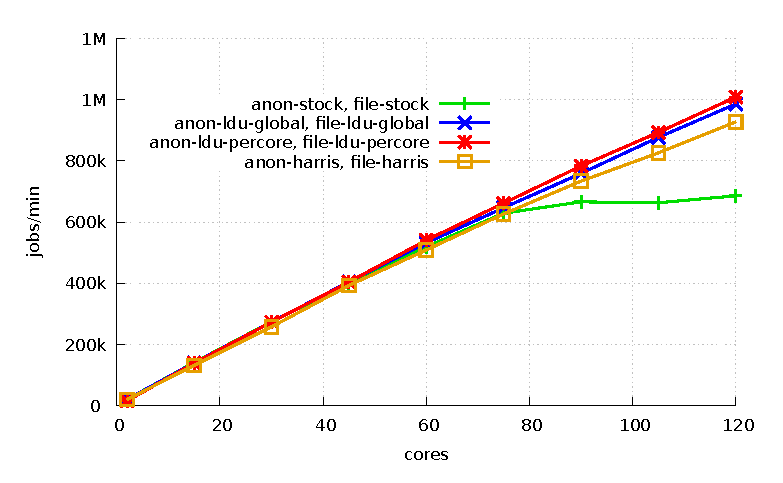
\includegraphics[scale=1]{graph/aim7.eps}
  \end{center}
  \caption{AIM7-multiuser 확장성.}
  \label{fig:aim7}
\end{figure}

\begin{figure*}[tb]
    \centering
    \begin{subfigure}[b]{1\textwidth}
  \begin{center}
        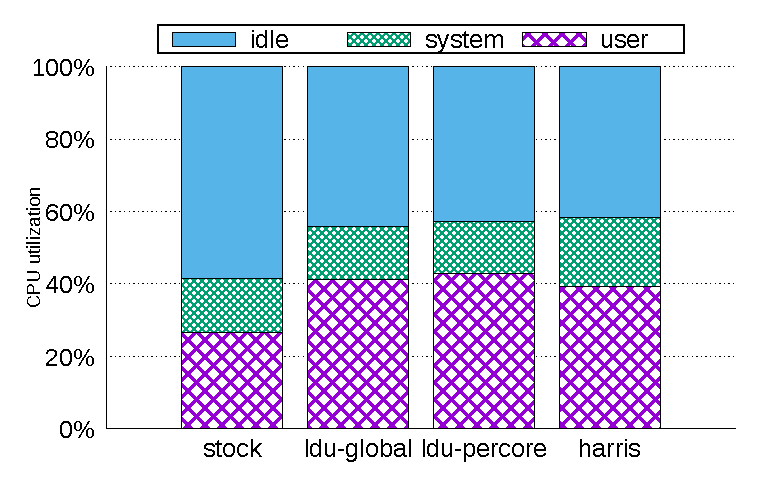
\includegraphics[scale=0.7]{graph/aim7_cpuutils.eps}
  \end{center}
    \end{subfigure}%
    \centering
    \caption{120코어에서 AIM7 CPU 사용량.}
    \label{fig:utilization_aim7}
    
\end{figure*}

\begin{figure*}[tb]
    \centering
    \begin{subfigure}[b]{1\textwidth}
  \begin{center}
        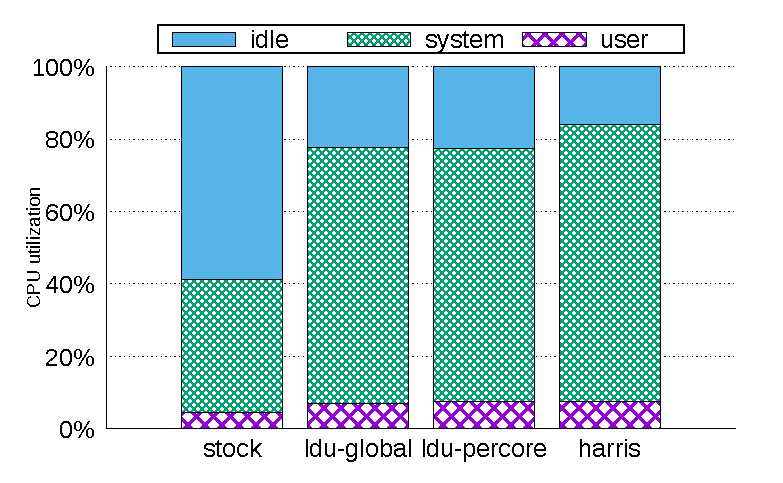
\includegraphics[scale=0.7]{graph/exim_cpuutils.eps}
  \end{center}
    \end{subfigure}
    \centering
    \caption{120코어에서 EXIM CPU 사용량. }
    \label{fig:utilization_exim}
    
\end{figure*}

\begin{figure*}[tb]
    \centering
    \begin{subfigure}[b]{1\textwidth}
  \begin{center}
        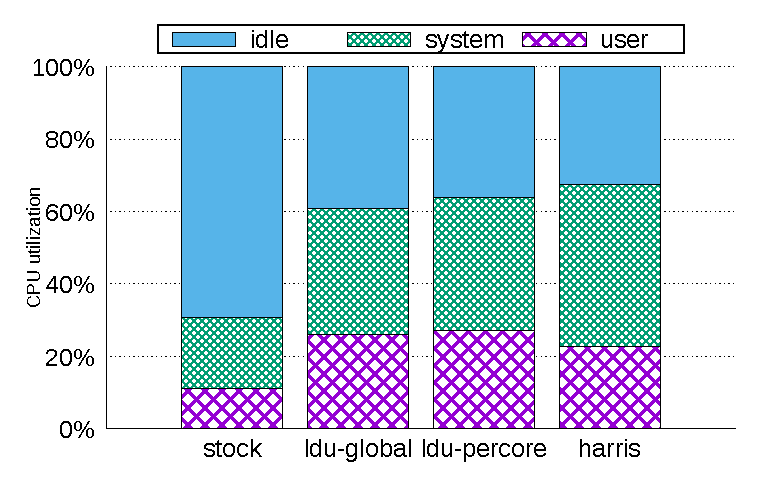
\includegraphics[scale=0.7]{graph/lmbench_cpuutils.eps}
  \end{center}
    \end{subfigure}
        \centering
    \caption{120코어에서 Lmbench CPU 사용량.}
    \label{fig:utilization_lmbench}
    
\end{figure*}

%$$$$$$$$$$$$$$$$$$$$$$$$$$$$$$$$$$$$$$$$$$$$$$$$$$$$$$$$$$$$$$$$$$$$$$$$$$$$$$$$
%Paragraph 1: AIM7 실험 결과
%$$$$$$$$$$$$$$$$$$$$$$$$$$$$$$$$$$$$$$$$$$$$$$$$$$$$$$$$$$$$$$$$$$$$$$$$$$$$$$$$


%$$$$$$$$$$$$$$$$$$$$$$$$$$$$$$$$$$$$$$$$$$$$$$$$$$$$$$$$$$$$$$$$$$$$$$$$$$$$$$$$
%Paragraph 1: 워크로드에 대한 설명
%$$$$$$$$$$$$$$$$$$$$$$$$$$$$$$$$$$$$$$$$$$$$$$$$$$$$$$$$$$$$$$$$$$$$$$$$$$$$$$$$
우리는 AIM7-multiuser를 사용하였다. 
이것은 AIM7의 워크로드 중 리눅스 \code{fork}에 집중된 벤치마크이다. 
이러한 multiuser 워크로드는 동시에 많은 프로세스를 생성 한 후 다양한 
일을 수행한다(see section~\ref{sec:bg}). 
또한 우리는 파일 시스템에 대한 병목현상을 줄이기 위해 리눅스 \code{tmpfs}를 사용하였다. 
또한 우리는 코어 수에 비례하여 AIM7의 입력 값인 유져 수를 증가하였다. 
 
%$$$$$$$$$$$$$$$$$$$$$$$$$$$$$$$$$$$$$$$$$$$$$$$$$$$$$$$$$$$$$$$$$$$$$$$$$$$$$$$$
%Paragraph 2: 실험 결과에 대한 설명
%$$$$$$$$$$$$$$$$$$$$$$$$$$$$$$$$$$$$$$$$$$$$$$$$$$$$$$$$$$$$$$$$$$$$$$$$$$$$$$$$
AIM7-multiuser에 대한 실험 결과는 그림 ~\ref{fig:aim7}과 같다.
75코어 전 까지는 수정 안한 리눅스는 확장성이 일정하나 그 이후에는 직렬화된 업데이트 
연산 때문에 병목 현상이 생긴다. 
하지만 120코어까지 Harris 링크드 리스트와 우리의 LDU는 확장성이 있다. 
그 이유는 워크로드들이 업데이트 명령어와 읽기-쓰기 세마포어(\code{anon\_vma->rwsem},
\code{mapping->i\_mmap\_rwsem}) 없이 동시 적으로 실행될 수 있기 때문이다.
LDU의 per-core 큐 버전은 가장 좋은 성능을 보여주고, 확장성도 뛰어나며, 
수정 안 한 리눅스에 비해 1.5배 빠르고 Harris보다 1.1x 빠르다.

게다가, 비록 LDU의 전역 큐 버전은 전역 CAS 명령어를 실행하지만, 이 방법 역시 높은 성능과 확장성을 가진다.
그 이유는 LDU의 2가지 기법 때문에 전역 CAS에 대한 접근이 완화되었기 때문이다.
이것은 퍼코어 버전에 비해 2\% 성능 저하가 생긴다. 
더욱이, 수정 안 한 리눅스는 가장 높은 유휴(IDLE) 시간(56\%)을 가진다(그림 ~\ref{fig:utilization_aim7}). 
그 이유는 2가지 세마포어(i.e.,
\code{anon\_vma->rwsem}, \code{mapping->i\_mmap\_rwsem}))를 얻기 위해 기다리기 때문이다.
비록 2가지 LDU가 Harris 커널 버전보다 높은 유휴시간을 가지지만, 처리량은 Harris 방법보다 더 높다.
이것은 바로 우리의 LDU 알고리즘이 효율적임을 보여준다. 

\begin{figure}[tb]
  \begin{center}
    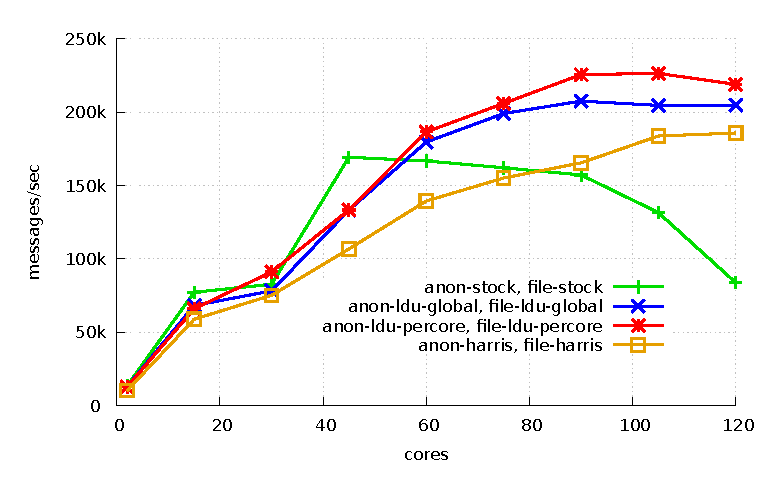
\includegraphics[scale=1]{graph/exim.eps}
  \end{center}
  \caption{Exim 확장성.}
  \label{fig:exim}
\end{figure}

\subsection{Exim}
%$$$$$$$$$$$$$$$$$$$$$$$$$$$$$$$$$$$$$$$$$$$$$$$$$$$$$$$$$$$$$$$$$$$$$$$$$$$$$$$$
%Paragraph 1:  EXIM 실험 결과
%$$$$$$$$$$$$$$$$$$$$$$$$$$$$$$$$$$$$$$$$$$$$$$$$$$$$$$$$$$$$$$$$$$$$$$$$$$$$$$$$

\begin{figure}[tb]
  \begin{center}
    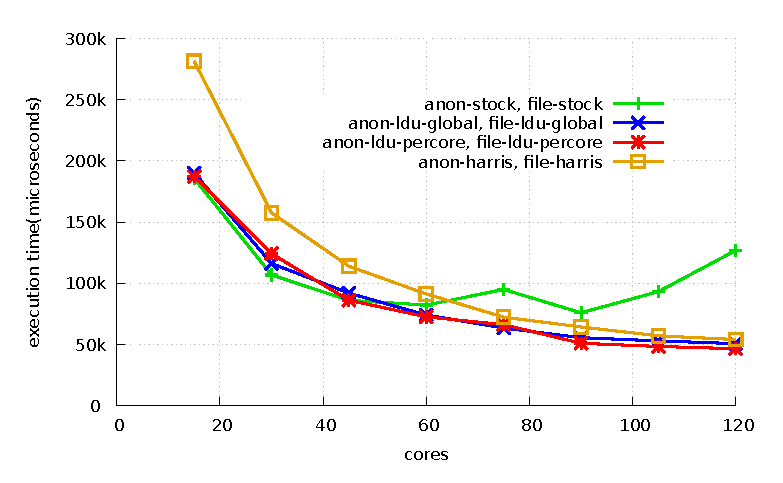
\includegraphics[scale=1]{graph/lmbench.eps}
  \end{center}
  \caption{Lmbench의 프로세스 관리 벤치마크에 대한 실행시간.}
  \label{fig:MicroBench}
\end{figure}

%$$$$$$$$$$$$$$$$$$$$$$$$$$$$$$$$$$$$$$$$$$$$$$$$$$$$$$$$$$$$$$$$$$$$$$$$$$$$$$$$
%Paragraph 1: 워크로드에 대한 설명
%$$$$$$$$$$$$$$$$$$$$$$$$$$$$$$$$$$$$$$$$$$$$$$$$$$$$$$$$$$$$$$$$$$$$$$$$$$$$$$$$
Exim의 성능에 대한 확장성을 측정하기 위하여, 우리는 매니코어 확장성 벤치마크 중 하나인 MOSBENCH를 이용하였다. 
이메일(E-mail) 서버인 Exim의 디자인은 확장성이 있게 설계되었다. 
그 이유는 Exim의 메시지(Message) 전달자(Delivers)는 리눅스의 프로세스 기반으로 
병렬 적인 방법을 사용하여 메시지를 메일 박스에 전달한다.
이러한 Exim은 \code{fork}가 많이 발생하는 워크로드 중 하나이다. 
클라이언트는 같은 장치에서 실행하였고, 
각각의 클라인언트는 메일 파일에 대해서 충돌을 막기 위해, 여러 유저에게 보낸다 
Exim은 파일 시스템에서 병목 현상이 발생된다~\cite{SilasBoydWickizer2010LinuxScales48}.
그 이유는 메시지의 바디가 각각의 유저 메일 파일에 추가되기 때문이다.
따라서 우리는 파일 시스템의 병목 지점을 제거하기 위해 분활 된 \textit{tmpfs}를 사용하였다. 

%$$$$$$$$$$$$$$$$$$$$$$$$$$$$$$$$$$$$$$$$$$$$$$$$$$$$$$$$$$$$$$$$$$$$$$$$$$$$$$$$
%Paragraph 2:실험 결과에 대한 설명
%$$$$$$$$$$$$$$$$$$$$$$$$$$$$$$$$$$$$$$$$$$$$$$$$$$$$$$$$$$$$$$$$$$$$$$$$$$$$$$$$
그림~\ref{fig:exim}에서 보여주는 Exim의 결과 수정안 한 리눅스 커널은 
60코어 까지 확장성이 좋게 동작을 한다. 
하지만 60코어 근처부터 성능이 떨어지는 모습을 볼 수 있다.
45코어 지점에서는 수정 안한 리눅스 커널이 성능이 높게 나오는데, 이것은 LDU가 사용하는 방법이 
궁극적으로 업데이트 연산을 뒤로 미루는 방법이기 때문에, 락 경합이 덜 발생하면 오히려 로깅하는 오버헤드 때문에 
성능이 떨어질 수 있다. 
이것은 LDU가 여전히 특정 워크로드와 함께 적은 코어에서의 문제점을 가지고 있다는 것을 보여준다.
하지만 60코어 이후에는 성능이 역전 되어 좋은 성능을 보인다. 

Harris와 LDU는 105코어까지 확장성을 보인다. 
그 이유는 이 두 방법은 세마포어 때문에 기다리는 현상이 없이 동시에 업데이트 연산이 가능하기 때문이다. 
LDU의 퍼코어 큐 버전은 보다 더 좋은 성능을 가진다.
그 이유는 이것은 캐시 일관성과 관련한 오버헤드를 줄였기 때문이며, 이것은 120코어에서 수정 안한 
리눅스보다 2.6배 성능 향상을 가지며 Harris 보다 1.2배의 성능 향상을 가진다.
비록 우리는 확장성이 있는 기술을 적용하였지만, Exim은 105코어부터 성능 확장성에 대해서 문제가 생긴다.
그 이유는 Exim의 프로세스들은 상대적으로 큰 크기의 가상 메모리를 사용하기 때문이다.
이것은 결국 프로세스가 종료될 때 가상 메모리에 대한 초기화 오버헤드를 낳으며,
결국 많은 소프트 페이지 폴트(Soft Page Fault)를 야기 시킨다. 
이것은 특히 NUMA 구조와 같은 구조에서는 원격 메모리를 접근하는 현상 때문에 더욱 많은 오버헤드를 가진다.
Harris 링크드 리스트는 15\%의 유휴 시간을 가진 반면, per-core 큐 버전의 LDU는 22\%의 유휴 시간을 가진다.
그 이유는 LUD의 효율적인 알고르즘 때문이다(그림~\ref{fig:utilization_exim}).

\subsection{Lmbench}
%$$$$$$$$$$$$$$$$$$$$$$$$$$$$$$$$$$$$$$$$$$$$$$$$$$$$$$$$$$$$$$$$$$$$$$$$$$$$$$$$
%Paragraph 1: %워크로드에 대한 설명
%$$$$$$$$$$$$$$$$$$$$$$$$$$$$$$$$$$$$$$$$$$$$$$$$$$$$$$$$$$$$$$$$$$$$$$$$$$$$$$$$
Lmbench는 다양한 마이크로(Micro) 벤치마크를 포함하고 있다. 
우리는 이러한 다양한 마이크로 벤치마크 중 프로세스 관리에 대한 워크로드를 사용하였다. 
이러한 워크로드는 기본적인 프로세스 관리에 대한 요소들인 프로세스 생성, 
프로그램 시작 그리고 문맥교환들에 대해서 성능을 측정한다.
그리고 우리는 프로세스 생성에 대한 워크로드에 대해 병렬 옵션 값인 1000을 사용하여 수행하였다. 

%$$$$$$$$$$$$$$$$$$$$$$$$$$$$$$$$$$$$$$$$$$$$$$$$$$$$$$$$$$$$$$$$$$$$$$$$$$$$$$$$
%Paragraph 2: 실험 결과에 대한 설명
%$$$$$$$$$$$$$$$$$$$$$$$$$$$$$$$$$$$$$$$$$$$$$$$$$$$$$$$$$$$$$$$$$$$$$$$$$$$$$$$$
Lmbench의 결과는 그림~\ref{fig:MicroBench}에서 보여주며, 세로축에 대한 결과는 실행 시간이다.
45코어까지, 수정 안 한 리눅스 커널은 일정한 확장성을 보이며, 그 이후 실행시간을 늘어난다.
퍼코어 버전의 LDU는 120코어에서 수정 안 한 리눅스 커널에 2.7배 성능향상으로 보이며, 
Harris 리스트에 비해 1.1배의 성능향상을 보인다.
수정 안 한 리눅스는 69\%의 유휴 시간을 가진 반면 다른 방법들은 약 35\% 정도의 유휴시간을 가진다.
그 이유는 수정 안한 리눅스 커널은 2가지 RMAP 세마포어(\code{anon\_vma->rwsem},
\code{mapping->i\_mmap\_rwsem})(figure~\ref{fig:utilization_lmbench})를 기다리기 때문이다. 
사실, 우리의 LDU에 대한 개발 동기는 120코어에서 성능과 확장성을 개선하는 것이다. 
따라서 우리는 적은 코어(30코어 이내)에서의 성능은 고려하지 않았었다
하지만 30코어까지 우리의 LDU는 수정 안한 리눅스 커널과 비슷한 성능을 보인다. 
반면, Harris 링크드 리스트는 60 코어 까지 안 좋은 성능을 보여준다. 
이러한 현상은 LDU의 효율적인 알고리즘 때문이다.

\subsection{업데이트 비율}

%$$$$$$$$$$$$$$$$$$$$$$$$$$$$$$$$$$$$$$$$$$$$$$$$$$$$$$$$$$$$$$$$$$$$$$$$$$$$$$$$
%Paragraph 2:  실험을 수행한 이유
%$$$$$$$$$$$$$$$$$$$$$$$$$$$$$$$$$$$$$$$$$$$$$$$$$$$$$$$$$$$$$$$$$$$$$$$$$$$$$$$$
본 논문에서 제안하는 LDU는 Update-heavy한 자료구조를 위한 방법이다. 
따라서 리더가 많아질 경우 성능이 떨어지는 단점을 가진다. 
그 이유는 LDU의 읽기 연산은 로그를 적용하는 \code{synchronize} 함수를 호출하므로, 
그 동안 쌓인 로그들을 적용하게 되는데 이 경우 \code{synchronize} 함수의 
추가적인 연산 때문에 읽기 연산이 많이 지면 성능이 떨어진다.
그러므로 우리가 제안하는 LDU에서의 하나의 의문 사항은 바로 읽기
연산이 자주 발생할 경우는 성능에 대한 확장성이 어떻게 될까? 이다.

읽기 연산에 대한 효과를 이해하기 위해 읽기 연산을 업데이트 연산의 비율에 
맞게 추가하여 성능을 측정하는 실험을 하였다.
실험을 단순화 하기 위해 익명 RMAP 자료 구조는 LDU의 전역 큐 버전을 이용하였고 
파일 RMAP에 대해서 순차적으로 읽기 연산(\code{lock}, \code{synchronize}) 비율을 증가 시켰다.
예를 들어 99\%는 파일 RMAP에 대해서 업데이트 연산이 99번 수행할 때 1번의 읽기 연산이 
일어나는 것을 의미하고, 순차적으로 90\%는 9번 업데이트에 1번의 읽기 연산을 의미한다.

\begin{figure}[h!]
    \centering
    \begin{subfigure}[b]{1\textwidth}
        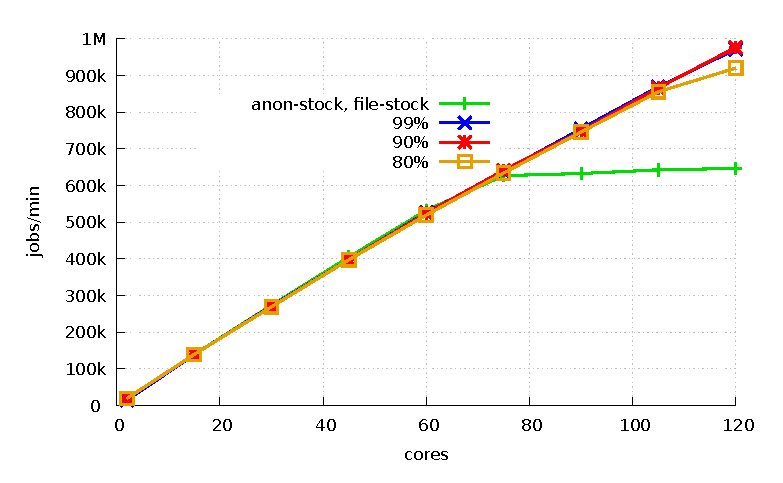
\includegraphics[height=2.5in]{graph/ratio_aim7_core.eps}
    \end{subfigure}%
    \caption{업데이트 비율에 따른 AIM7 확장성.}
    \label{fig:UpdateRate_aim7_2}
\end{figure}
 
 
%$$$$$$$$$$$$$$$$$$$$$$$$$$$$$$$$$$$$$$$$$$$$$$$$$$$$$$$$$$$$$$$$$$$$$$$$$$$$$$$$
%Paragraph 2: 실험 결과에 대한 설명
%$$$$$$$$$$$$$$$$$$$$$$$$$$$$$$$$$$$$$$$$$$$$$$$$$$$$$$$$$$$$$$$$$$$$$$$$$$$$$$$$
그림~\ref{fig:UpdateRate_aim7_2}는 AIM7의 실험 결과를 보여준다.
다른 2가지 벤치마크(Exim, Lmbench) 비해 덜 \code{fork}에 의존적인 벤치마크이기 때문에, 
읽기 연산이 호출되는 간격이 상대적으로 짧다.
그 결과, 비록 자료구조가 80\%의 업데이트 비율(4개의 업데이트 연산 일때 1개의 읽기 연산을 수행)을 
가지지만, LDU의 버전의 리눅스는 수정 안 한 리눅스에 비해 높은 성능을 가진다. 
AIM7의 성능에 대한 확장성은 90\% 이상의 뿐만 아니라 80\%의 업데이트 비율을 가질 때에도 수정안 한 
리눅스 보다 높은 성능 확장성을 가진다.
 
\begin{figure}[h!]
    \centering
    \begin{subfigure}[b]{1\textwidth}
        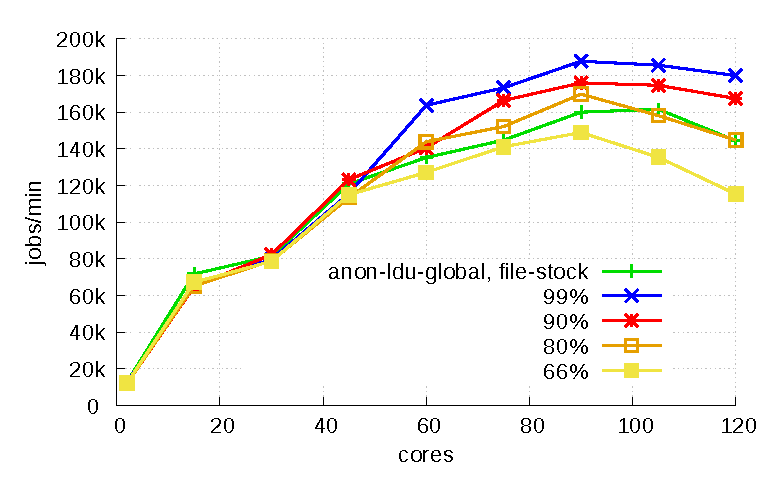
\includegraphics[height=2.5in]{graph/ratio_exim_core.eps}
    \end{subfigure}%
    \caption{업데이트 비율에 따른 Exim 확장성.}
    \label{fig:UpdateRate_exim_2}
\end{figure}


%$$$$$$$$$$$$$$$$$$$$$$$$$$$$$$$$$$$$$$$$$$$$$$$$$$$$$$$$$$$$$$$$$$$$$$$$$$$$$$$$
%Paragraph 2: 실험 결과에 대한 설명
%$$$$$$$$$$$$$$$$$$$$$$$$$$$$$$$$$$$$$$$$$$$$$$$$$$$$$$$$$$$$$$$$$$$$$$$$$$$$$$$$
Exim과 매우 \code{fork}를 많이 호출하는 워크로드 중 하나이다. 
따라서 업데이트 연산이 빨리 호출되는 특징을 가지며, 동시에 읽기 연산의 간격도 짧다는 것이다. 
즉 AIM7과는 다르게 \code{synchronize} 함수가 자주 호출된다는 것을 의미한다.
그 결과, 80\% 이하의 업데이트 연산 비율을 가지면 수정안한 리눅스 보다 더 안 좋은 성능을 가진다.
LDU는 90\% 이상의 업데이트 가질 때부터 더 높은 성능을 가진다.

\begin{figure}[h!]
    \centering
    \begin{subfigure}[b]{1\textwidth}
        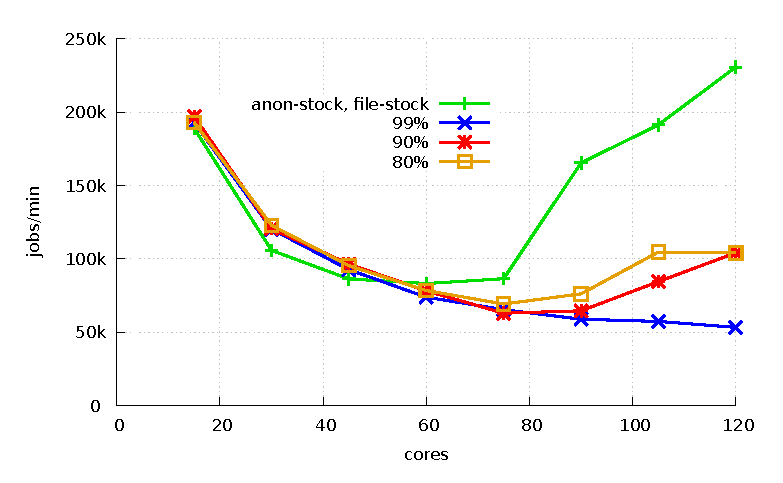
\includegraphics[height=2.5in]{graph/ratio_lmbench_core.eps}
    \end{subfigure}%
    \caption{업데이트 비율에 따른 Lmbench 확장성.}
    \label{fig:UpdateRate_lmbench_2}
\end{figure}

%$$$$$$$$$$$$$$$$$$$$$$$$$$$$$$$$$$$$$$$$$$$$$$$$$$$$$$$$$$$$$$$$$$$$$$$$$$$$$$$$
%Paragraph 2: 실험 결과에 대한 설명
%$$$$$$$$$$$$$$$$$$$$$$$$$$$$$$$$$$$$$$$$$$$$$$$$$$$$$$$$$$$$$$$$$$$$$$$$$$$$$$$$
Lmbench는 Exim과 비슷하게 \code{fork}가 자주 호출 되는 워크로드이다.
Lmbench는 실행 시간을 보여주므로, 낮을 수록 높은 성능을 보여준다. 
실험 결과 Exim과 비슷한 결과를 보이는데, 이것은 수정안한 리눅스가 80\%의 업데이트 
비율을 가질 때 더 좋은 성능을 가진다.
하지만 Lmbench는 굉장히 \code{fork}가 자주 호출되는 마이크로 벤치마크이기 때문에 업데이트 연산의 비율이 
90\%가 되면 비록 수정 안한 리눅스 보다는 성능이 좋지만, 확장성이 떨어지는 특징을 가진다.
하지만 LUD는 읽기가 상당히 자주 호출되는 워크로드라도 업데이트 비율이 90\% 이상이면 
좋은 성능을 보여준다는 것을 설명한다. 
 


\chapter{결론 및 향후 연구}\label{sec:concl}

\section{결론}

우리는 동시적 업데이트 방법인 LDU를 개발하였고, 
이것을 매니코어 시스템에 적용하여 성능 확장성을 보였다.
LDU는 기존 로그 기반 알고리즘 중 하나인 OpLog의 동기화된 타임스템프 카운터를 완벽히 제거 할 수 있다. 
우리는 이러한 LDU를 최신 리눅스 커널에 구현하였고, 실험 결과 기존 리눅스 커널에 비해 2.7배까지 성능 향상을 이루었다. 

이처럼 동기화된 타임 스탬프 카운터를 제거함과 동시에, 캐시 커뮤니케이션 병목 현상을 줄인
LDU는 기존 로그 기반 알고리즘들의 장점을 모두 포함할 뿐만 아니라 추가적인 장점을 가진다.
첫째, 업데이트가 수행하는 시점 즉 로그를 저장하는 순간에는 락이 필요가 없다.
따라서 락의 오버헤드 없이 동시적 업데이트를 수행할 수 있다.
둘째로, 저장된 업데이트 연산들의 로그를 하나의 코어에서 수행되기 때문에, 
캐시 효율성이 높아진다.
다음으로, 기존 여러 자료구조에 쉽게 적용할 수 있는 장점이 있다.
게다가 마지막으로, 로그를 저장하기 전에 로그를 쉽게 삭제하므로 성능을 높일 수 있다. 

LDU는 동기화된 타임 스탬프 카운터를 제거하기 위해, 타임 스탬프 카운터가 반드시 필요한 연산들은 
업데이트 순간 제거하고 매번 로그를 생성하지 않고 재활용하는 방법을 사용하였다.
이로 인해 동기화된 타임스탬프 카운터의 현실적인 구현 문제와 캐시 일관성 트래픽 때문에 발생하는 
병목 현상 문제를 동시에 해결하였다.

우리는 이러한 LDU를 리눅스 커널 4.5-rc6에 구현하였으며, 결과물은
아래 사이트에서 오픈소스로 이용할 수 있다.
\begin{center}
\url{https://github.com/manycore-ldu/ldu}
\end{center}

\newpage
\section{향후 연구}

우리가 제안한 기술은 로그 기반 방법 중 하나이다. 
아직 하드웨어 적으로 지원하지 않고, 소프트웨어들로도 검증되지 않은 
동기화된 타임 스탬프 카운터를 사용하지 않았고, 순서가 중요한 로그들을 업데이트 순간 마다 지우는 방법을 사용하였다. 
하지만, 여전히 스왑이라는 명령어로 공유 데이터를 수정한다.

향후 연구로 OpLog와 같이 타임 스탬프 기법을 사용할 수 있도록, 
여러 하드웨어 환경에서도 지원할 수 있는 소프트웨어 기반의 동기화된 타임 스탬프 카운터를 구현하는 것이다.
또한 업데이트 순간 락을 제거하고, 삭제 가능한 로그들을 제거함으로 
성능에 대한 향상 성을 얻었으나, 읽기 연산이 증가할 수 록 성능이 많이 떨어지는 것을 볼 수 있다.
그러므로 다른 향후 연구 방향으로는 로그 기반 기술을 다른 동기화 기법과 통합하는 것이다. 
예를 들어 RCU와 같은 기법은 읽기 연산이 많을 수록 굉장히 높은 성능을 보여준다.
이처럼 RCU의 업데이트 부분을 수정하여, 로그 기반으로 작성하는 연구가 필요하다.
결론적으로 여러 동기화 기술을 통합한 새로운 동기화 기법을 개발하는 것이 필요하다.



%\begin{thebibliography}{1}
%\bibliographystyle{IEEEtran}
\bibliographystyle{alpha}
%\bibliography{ref}
\bibliography{ref}
%\end{thebibliography}


\newpage
\addcontentsline{toc}{content}{Abstract}% 목차(TOC)에 추가
\hfill \break

\noindent
\Large{\textbf{Abstract}}

\noindent
\Large{\textbf{A Lightweight Log-based Deferred Update for Linux Kernel
Scalability}}

\normalsize{
\hfill \break
\begin{center}
\raggedleft{\textit{by Kyong, Joohyun}}\\
\raggedleft{\textit{Department of Computer Science}}\\
\raggedleft{\textit{Graduate School, Kookmin University,}}\\
\raggedleft{\textit{Seoul, Korea}}
\end{center}
\hfill \break

In highly parallel computing systems with many-cores, a few critical factors
cause performance bottlenecks severely limiting scalability.
The kernel data structures with high update rate naturally cause performance
bottlenecks due to very frequent locking of the data structures.
There have been research on log-based synchronizations with time-stamps that
have achieved significant level of performance and scalability improvements.
However, NUMA-based modern processors have not provided the
practical global synchronized time-stamp counters.

To overcome the practical problem of the synchronized time-stamp counters, we
introduce a lightweight log-based deferred update method, combining the
log-based concepts in the distributed systems and the minimal hardware-based
synchronization in the shared memory systems.
The main contributions of the proposed method are:(1) we propose a lightweight
log-based deferred update method, which can eliminate synchronized time-stamp
counters;and (2) we implemented the proposed method in the Linux 4.5-rc6 kernel
for two representative data structures (anonymous reverse mapping and file
mapping) and evaluated the performance improvement due to our proposed novel
light weight update method.
Our evaluation study showed that application of our method could
achieve from 1.5x through 2.7x performance improvements in 120 core
systems.}

%% 본문 끝
\end{document}
